\documentclass[conference]{IEEEtran}
\usepackage{amsmath,amsthm}
\usepackage[T1]{fontenc}
\usepackage{newtxtext,newtxmath}
\usepackage{graphicx,booktabs,multirow,xcolor}
\usepackage{algorithm,algpseudocode}
\usepackage[hidelinks]{hyperref}
\usepackage{cite}
\usepackage{microtype}
\usepackage{tikz}
\usetikzlibrary{arrows.meta,positioning}

\newtheorem{theorem}{Theorem}
\newtheorem{lemma}{Lemma}
\newtheorem{proposition}{Proposition}
\newtheorem{corollary}{Corollary}
\theoremstyle{definition}
\newtheorem{definition}{Definition}

\newcommand{\R}{\mathbb{R}}
\newcommand{\norm}[1]{\left\lVert #1 \right\rVert}
\newcommand{\gm}{\operatorname{GM}}
% Generated by make_numbers.py from experiments/foa/results. Do not edit.
\newcommand{\AblDiscardFPR}{54\%}
\newcommand{\AblFOAFPR}{7.0\%}
\newcommand{\AblFullComp}{67\%}
\newcommand{\AblMeanLamFPR}{13.8\%}
\newcommand{\AblNoPeersFPR}{43\%}
\newcommand{\AutoBoundaryComp}{63\%}
\newcommand{\AutoBoundaryCompHigh}{84\%}
\newcommand{\AutoComp}{39.2\%}
\newcommand{\AutoFleetFPR}{24.6\%}
\newcommand{\AutoIdioFPR}{26\%}
\newcommand{\AutoMedTTC}{30}
\newcommand{\BoundViolations}{0}
\newcommand{\ByzAloneMax}{0\%}
\newcommand{\ByzAuto}{80\%}
\newcommand{\ByzF}{100\%}
\newcommand{\ByzH}{100\%}
\newcommand{\ByzO}{0\%}
\newcommand{\ByzT}{0\%}
\newcommand{\ByzTF}{60\%}
\newcommand{\ByzTH}{56\%}
\newcommand{\ByzTO}{2\%}
\newcommand{\ByzTT}{40\%}
\newcommand{\ByzTZ}{0\%}
\newcommand{\ByzV}{100\%}
\newcommand{\ByzZ}{0\%}
\newcommand{\CesAutoComp}{18\%}
\newcommand{\CesAutoFPR}{11.6\%}
\newcommand{\CesFOAComp}{0\%}
\newcommand{\CesFOAFPR}{9.1\%}
\newcommand{\CesFrozenComp}{0\%}
\newcommand{\CesFrozenFPR}{11.6\%}
\newcommand{\CesKLComp}{18\%}
\newcommand{\CesKLFPR}{13.3\%}
\newcommand{\CesNaiveComp}{91\%}
\newcommand{\CesNaiveFPR}{5.2\%}
\newcommand{\CesStaticFPR}{5.9\%}
\newcommand{\ExplainedVar}{93.2\%}
\newcommand{\FOABoundaryComp}{0\%}
\newcommand{\FOAComp}{10.8\%}
\newcommand{\FOACoreHigh}{34\%}
\newcommand{\FOAFleetFPR}{9.0\%}
\newcommand{\FOAFreezeClean}{11.8\%}
\newcommand{\FOAFreezeFPR}{11.8\%}
\newcommand{\FOAIdioFPR}{36\%}
\newcommand{\FOAMedTTC}{64}
\newcommand{\FOAMimicHigh}{29\%}
\newcommand{\FlAutoCompBound}{63.2\%}
\newcommand{\FlAutoCompNone}{7.4\%}
\newcommand{\FlAutoCompStrong}{39.2\%}
\newcommand{\FlAutoFCompBound}{75.4\%}
\newcommand{\FlAutoFCompNone}{7.6\%}
\newcommand{\FlAutoFCompStrong}{43.1\%}
\newcommand{\FlAutoFIdioFPR}{0.9\%}
\newcommand{\FlAutoFModFPR}{0.9\%}
\newcommand{\FlAutoFStrongFPR}{0.8\%}
\newcommand{\FlAutoIdioFPR}{20.3\%}
\newcommand{\FlAutoModFPR}{18.9\%}
\newcommand{\FlAutoStrongFPR}{24.6\%}
\newcommand{\FlFOACompBound}{0.0\%}
\newcommand{\FlFOACompNone}{4.6\%}
\newcommand{\FlFOACompStrong}{10.8\%}
\newcommand{\FlFOAFCompBound}{0.0\%}
\newcommand{\FlFOAFCompNone}{4.3\%}
\newcommand{\FlFOAFCompStrong}{9.4\%}
\newcommand{\FlFOAFIdioFPR}{24.6\%}
\newcommand{\FlFOAFModFPR}{1.4\%}
\newcommand{\FlFOAFStrongFPR}{2.5\%}
\newcommand{\FlFOAIdioFPR}{28.2\%}
\newcommand{\FlFOAModFPR}{6.0\%}
\newcommand{\FlFOAStrongFPR}{9.0\%}
\newcommand{\FourCompAuto}{75\%}
\newcommand{\FourCompFOA}{0\%}
\newcommand{\FourCompFrozen}{0\%}
\newcommand{\FourCompKL}{50\%}
\newcommand{\FourCompStatic}{n/a}
\newcommand{\FourFPRAuto}{29\%}
\newcommand{\FourFPRFOA}{11\%}
\newcommand{\FourFPRFrozen}{77\%}
\newcommand{\FourFPRKL}{51\%}
\newcommand{\FourFPRStatic}{100\%}
\newcommand{\FrozenComp}{27.4\%}
\newcommand{\GateFleetFPR}{45\% to 59\%}
\newcommand{\JoinComp}{0\%}
\newcommand{\KLCleanFPR}{26\%}
\newcommand{\KLComp}{29.9\%}
\newcommand{\KLFrozenFPR}{100\%}
\newcommand{\LossHalfFPR}{6.7\%}
\newcommand{\LossNoneFPR}{6.4\%}
\newcommand{\MonoCiotaOne}{0\%}
\newcommand{\MonoCiotaThree}{100\%}
\newcommand{\MonoFOAThree}{0\%}
\newcommand{\MonoSameThree}{100\%}
\newcommand{\NRunsEThree}{6{,}720}
\newcommand{\NaiveFleetFPR}{2.6\%}
\newcommand{\NoDriftAutoComp}{7\%}
\newcommand{\NoDriftFOAComp}{5\%}
\newcommand{\NoDriftNaiveComp}{36\%}
\newcommand{\ORFrozenFPR}{26\%}
\newcommand{\StrongStaticFPR}{78\%}
\newcommand{\SweepCompHigh}{75\%}
\newcommand{\SweepIdioHigh}{11\%}
\newcommand{\SweepIdioLow}{55\%}
\newcommand{\SweepSafeMaxB}{0.005}
\newcommand{\SweepViol}{0}
\newcommand{\SybilFOA}{0\%}
\newcommand{\SybilNoHMAC}{100\%}
\newcommand{\TOAComp}{5.5\%}


\begin{document}

\title{Fleet-Orthogonal Adaptation: Poison-Resilient\\On-Device Intrusion Detection for Drifting IoT\\\large Extended Edition}

\author{\IEEEauthorblockN{Rishit Kamboj and Farhan Naik}
\IEEEauthorblockA{Department of Computer Science and Engineering, Shiv Nadar University\\
CSD457 Internet of Things, Group G-04}}

\maketitle

\begin{abstract}
An intrusion detector that runs on an IoT device must keep learning, because normal traffic drifts. But
a detector that labels its own traffic can be walked toward an attack by a slow poisoner, and a defence
that stops learning when traffic looks suspicious can be frozen by an attacker who trips it and leaves.
From a single device's stream, honest drift and slow poisoning cannot be told apart. We observe that IoT
devices rarely live alone: most honest drift is shared by a device's neighbours, while a poisoning
campaign reaches only the devices its exploit reaches. Fleet-Orthogonal Adaptation (FOA) gives each
device a robust consensus of vulnerability-diverse peers, exchanged as 92-byte authenticated ESP-NOW
frames: the part of a device's update its peers back is applied in full, and the device-specific rest
passes through a budget that never closes. We prove that an attacker on one device gains at most
$B_0+Bt$ alarm radii of movement, that key-holding Byzantine peers add a bounded bias per cycle, that
FOA has no freeze state, and that device-only drift and poisoning are indistinguishable for any rule.
On all nine N-BaIoT devices with real Mirai and BASHLITE traffic, under strong shared drift, FOA keeps
fleet false alarms at \FOAFleetFPR\ (single-device adaptation \AutoFleetFPR, gated defences
\GateFleetFPR) while cutting attack-attributable compromise from \AutoComp\ to \FOAComp; it is never
compromised by the classic boundary poisoner, resists a monoculture botnet that defeats same-model
consensus, and is unaffected by a freeze attack that locks an alarm-rate switch-off at
\KLFrozenFPR\ false alarms. On 40 weeks of real CESNET traffic it is never compromised. On three real
ESP8266 boards FOA gossips reliably at about 15\,ms of computing per cycle, but identical boards shrank
their detectors together until false alarms reached 90\%. A coverage floor removes this in simulation
(strong-drift false alarms \FlFOAFStrongFPR) and revises our claim: with the floor a single device raises
no more false alarms than FOA, but is compromised in \FlAutoFCompStrong\ of attacked runs under drift
against FOA's \FlFOAFCompStrong.


This extended edition adds background on IoT attacks and attacker motives, a worked hospital example of slow poisoning, research questions and hypotheses, the full comparison against every baseline including a CIoTA-style rule, what FOA borrows from each prior work, the research journey, and a reference of every formula.
\end{abstract}

\begin{IEEEkeywords}
IoT security, intrusion detection, data poisoning, concept drift, on-device learning, robust aggregation, ESP32
\end{IEEEkeywords}

% Overview of Fleet-Orthogonal Adaptation (TikZ). Included by body.tex.
\begin{figure*}[t]
\centering
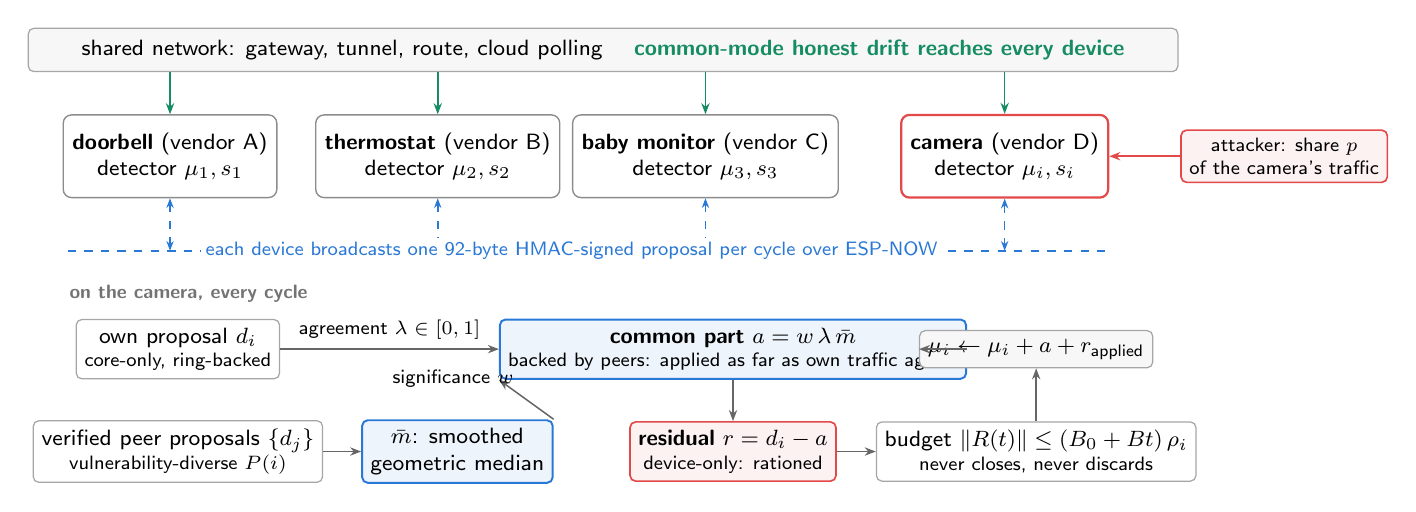
\begin{tikzpicture}[
  font=\sffamily\footnotesize,
  dev/.style={draw=black!45, rounded corners=3pt, fill=white, minimum width=2.55cm, minimum height=1.05cm, align=center, line width=0.5pt},
  box/.style={draw=black!35, rounded corners=2pt, fill=white, align=center, inner sep=3pt, line width=0.45pt},
  hero/.style={draw=foablue, rounded corners=2pt, fill=foablue!8, align=center, inner sep=3pt, line width=0.7pt},
  warn/.style={draw=atkred, rounded corners=2pt, fill=atkred!7, align=center, inner sep=3pt, line width=0.6pt},
  arr/.style={-{Stealth[length=4pt]}, line width=0.55pt, draw=black!60},
  gos/.style={{Stealth[length=3.5pt]}-{Stealth[length=3.5pt]}, line width=0.55pt, draw=foablue, dashed},
]
\definecolor{foablue}{HTML}{2A78D6}
\definecolor{atkred}{HTML}{E34948}
\definecolor{drift}{HTML}{1BAF7A}

% shared network and drift
\node[box, minimum width=14.6cm, minimum height=0.55cm, fill=black!3] (net) at (-0.5,2.35) {shared network: gateway, tunnel, route, cloud polling \quad
  \textcolor{drift!80!black}{\textbf{common-mode honest drift reaches every device}}};

% devices
\node[dev] (d1) at (-6.0,1.0) {\textbf{doorbell} (vendor A)\\ detector $\mu_1,s_1$};
\node[dev] (d2) at (-2.6,1.0) {\textbf{thermostat} (vendor B)\\ detector $\mu_2,s_2$};
\node[dev] (d3) at (0.8,1.0) {\textbf{baby monitor} (vendor C)\\ detector $\mu_3,s_3$};
\node[dev, draw=atkred, line width=0.8pt] (dv) at (4.6,1.0) {\textbf{camera} (vendor D)\\ detector $\mu_i,s_i$};
\foreach \d in {d1,d2,d3,dv} \draw[arr, draw=drift!80!black] (net.south -| \d.north) -- (\d.north);
\node[warn, font=\sffamily\scriptsize] (atk) at (8.15,1.0) {attacker: share $p$\\of the camera's traffic};
\draw[arr, draw=atkred] (atk.west) -- (dv.east);

% gossip bus
\draw[foablue, dashed, line width=0.6pt] (-7.3,-0.2) -- (5.9,-0.2);
\foreach \d in {d1,d2,d3,dv} \draw[gos] (\d.south) -- (\d.south |- 0,-0.2);
\node[font=\sffamily\scriptsize, text=foablue, fill=white, inner sep=1.5pt] at (-0.9,-0.2) {each device broadcasts one 92-byte HMAC-signed proposal per cycle over ESP-NOW};

% FOA pipeline on the attacked device
\node[font=\sffamily\scriptsize\bfseries, text=black!55, anchor=west] at (-7.4,-0.75) {on the camera, every cycle};
\node[box] (prop) at (-5.9,-1.45) {own proposal $d_i$\\[-1pt]{\scriptsize core-only, ring-backed}};
\node[box] (gm) at (-5.9,-2.75) {verified peer proposals $\{d_j\}$\\[-1pt]{\scriptsize vulnerability-diverse $P(i)$}};
\node[hero] (cons) at (-2.35,-2.75) {$\bar m$: smoothed\\geometric median};
\node[hero] (common) at (1.15,-1.45) {\textbf{common part} $a=w\,\lambda\,\bar m$\\[-1pt]{\scriptsize backed by peers: applied as far as own traffic agrees}};
\node[warn] (res) at (1.15,-2.75) {\textbf{residual} $r=d_i-a$\\[-1pt]{\scriptsize device-only: rationed}};
\node[box] (bud) at (5.0,-2.75) {budget $\lVert R(t)\rVert\le(B_0+Bt)\,\rho_i$\\[-1pt]{\scriptsize never closes, never discards}};
\node[box, fill=black!3] (upd) at (5.0,-1.45) {$\mu_i \leftarrow \mu_i + a + r_{\text{applied}}$};

\draw[arr] (prop.east) -- node[above, font=\sffamily\scriptsize]{agreement $\lambda\in[0,1]$} (common.west);
\draw[arr] (gm.east) -- (cons.west);
\draw[arr] (cons.north east) -- node[above left, font=\sffamily\scriptsize, pos=0.55]{significance $w$} (common.south west);
\draw[arr] (common.south) -- (res.north);
\draw[arr] (common.east) -- (upd.west);
\draw[arr] (res.east) -- (bud.west);
\draw[arr] (bud.north) -- (upd.south);
\end{tikzpicture}
\caption{Fleet-Orthogonal Adaptation. Every device runs its own detector and broadcasts its proposed
update each cycle. On each device, the part of its proposal that a robust consensus of
vulnerability-diverse peers backs is applied as far as the device's own traffic agrees; the
device-specific remainder, which is where a
single-device poisoning campaign lives, passes through a cumulative budget that grows forever, so
no gate switches learning off and the attacker's extra movement is bounded.}
\label{fig:system}
\end{figure*}

\section{Introduction}

Intrusion detection is moving onto IoT devices themselves: a detector that runs on the device sees its
traffic first, needs no upstream collector, and keeps working when the network is cut off. Such a
detector has to keep learning, because normal traffic does not stand still. Gateways change, tunnels add
bytes, cloud services change how often they poll, firmware updates change what a device sends. A
detector frozen at deployment drowns in false alarms within weeks.

Learning on the device has a well-known weak point. The detector labels its own traffic: whatever it
does not alarm on becomes the new normal. An attacker who controls part of that traffic can move the
boundary a little at a time until an attack looks normal, the boiling-frog attack~\cite{antidote,kloft}.
The obvious defence, stop learning when traffic looks suspicious, creates a second weakness that we
call the \emph{freeze attack}: an attacker trips the stop condition with loud traffic and leaves, honest
drift continues, and the frozen detector raises false alarms for good. Recent theory shows the dilemma
runs deeper: from a single label-free stream, honest drift and slow contamination can be made
indistinguishable~\cite{warden,capture}.

\textbf{Our observation} is that IoT devices rarely live alone. A doorbell, a thermostat and a camera on
the same network experience the same gateway, the same tunnel, the same polling changes: most honest
drift is \emph{common-mode}. A poisoning campaign, in contrast, reaches only the devices the attacker
can exploit, and devices from different vendors do not share exploits. The fleet is a second witness
that a single device does not have.

\textbf{Fleet-Orthogonal Adaptation (FOA)} turns that observation into an update rule
(Figure~\ref{fig:system}). Every device keeps its own detector and, each cycle, broadcasts its proposed
update as a 92-byte authenticated ESP-NOW frame. On each device the part of its proposal that a robust
consensus of vulnerability-diverse peers backs is applied, scaled by how far the device's own traffic
agrees; the device-specific remainder,
where a single-device campaign lives, passes through a cumulative budget that grows forever. Nothing is
discarded and no gate ever switches learning off, so a freeze attack has no stop condition to trip.

\textbf{Contributions.}
\begin{itemize}
\item \textbf{FOA}, a gate-free, label-free update rule that splits each on-device update into a
  peer-backed common part and a budgeted residual, with agreement measured robustly so that an attacker
  holding less than half a device's traffic can neither cancel nor fake it (Section~\ref{sec:design}).
\item \textbf{Guarantees}: the attacker's extra movement is bounded by $B_0+Bt$ alarm radii, giving a
  minimum time to compromise; $f<K/2$ key-holding Byzantine peers add only a bounded bias per cycle (and
alone never compromised a device in our runs); no
  gate stops learning; and a proof that device-only drift and poisoning cannot be separated by any
  rule, so FOA's single rate $B$ is the honest place to put the trade-off (Section~\ref{sec:theory}).
\item \textbf{Evaluation on all nine N-BaIoT devices} with real Mirai and BASHLITE traffic, physically
  modelled drift, eight baselines and held-out seeds. Under strong shared drift FOA cuts
  attack-attributable compromise from \AutoComp\ to \FOAComp\ (Section~\ref{sec:eval}); its lower false
  alarms there (\FOAFleetFPR\ against \AutoFleetFPR) do not survive the coverage floor of
  Section~\ref{sec:floor}.
\item \textbf{The freeze attack} on stop-learning gates: decoys leave FOA's trajectory bit-for-bit
  unchanged while they lock an alarm-rate switch-off at \KLFrozenFPR\ false alarms.
\item \textbf{Real drift} on 40 weeks of CESNET traffic~\cite{cesnet}, and \textbf{a C
  implementation} (compiled for the ESP32, run on three ESP8266 boards) that matches the reference on every recorded cycle, rejects all tampered frames and
  adds about 22\,KB of flash.
\item \textbf{Hardware lesson and a correction}: a three-board testbed exposed a spread collapse, a
  calibration aliasing bug and a stall after an abrupt change; a coverage floor fixes the collapse in
  simulation and on the boards and shows that FOA's lasting advantage is safety under drift
  rather than false alarms (Section~\ref{sec:hw}).
\end{itemize}

\section{Background: Attacks on IoT Devices}\label{sec:background}

This section sets out the starting point for readers new to IoT security: what an attack is, why anyone
attacks a thermostat or an infusion pump, what they gain, and which attacks matter for a detector that
learns on the device.

\subsection{What is an attack?}
An \emph{attack} is a deliberate action that makes a system behave against the wishes of its owner. Security
is usually stated as three properties, and every attack breaks at least one of them:
\begin{itemize}
\item \textbf{Confidentiality}: only authorised parties can read data (broken by data theft or eavesdropping).
\item \textbf{Integrity}: data and behaviour change only in authorised ways (broken by tampering, forged
  messages, or poisoning a model).
\item \textbf{Availability}: the system works when needed (broken by denial of service, or by a detector
  that drowns its operators in false alarms).
\end{itemize}
An attack needs a \emph{vulnerability} (a weakness such as a default password or a firmware bug) and an
\emph{exploit} (the method that uses it). The attacker's \emph{capabilities} (what they can see and
control) and \emph{goal} together form a \emph{threat model}; ours is stated in Section~\ref{sec:threat}.

\subsection{Why IoT devices are attacked}
IoT devices are attractive targets for five reasons. They are \emph{numerous}, so even a rare weakness
yields many victims. They are \emph{weakly protected}: default credentials, rarely patched firmware and
little memory for security software. They are \emph{always on and always connected}, which makes them
useful as relays. They \emph{sit inside trusted networks}, so a compromised camera is a foothold next to
laptops and servers. And some of them \emph{act on the physical world}: locks, pumps, beds and industrial
controllers. The Mirai botnet showed the scale: by scanning for default passwords it recruited a peak of
about 600,000 devices and used them for some of the largest denial-of-service attacks recorded at the
time~\cite{mirai}.

\subsection{What an attacker gains}
Table~\ref{tab:gains} lists the main motives. Most of them need the attacker to stay on the device for a
long time without being noticed, which is exactly why poisoning the device's own detector is worth the
effort.

\begin{table}[t]
\caption{What an attacker can gain from a compromised IoT device}\label{tab:gains}
\centering\footnotesize
\begin{tabular}{@{}p{2.1cm}p{5.9cm}@{}}
\toprule
Goal & Example and gain \\
\midrule
Botnet recruitment & Device floods a target on command; denial of service sold for hire \\
Data theft & Camera footage, health readings, patient identifiers; sold or used for fraud \\
Surveillance & Live audio or video from inside a home, office or ward \\
Extortion & Device or network locked until a ransom is paid \\
Lateral movement & Device used as a stepping stone into the hospital or company network \\
Sabotage & Wrong dose, unlocked door, stopped production line \\
Resource theft & Device used for cryptocurrency mining or as an anonymising proxy \\
\bottomrule
\end{tabular}
\end{table}

\subsection{Types of attack}
Table~\ref{tab:attacks} groups the attacks relevant to this paper. The first group attacks the device or
the network; it is what an intrusion detector is built to catch. Our evaluation uses real traffic of this
group from N-BaIoT~\cite{nbaiot}: the Mirai and BASHLITE botnets scanning for victims and flooding
targets with ACK, SYN, UDP, TCP and junk traffic. The second group attacks the \emph{detector itself}; it
is the subject of this paper.

\begin{table}[t]
\caption{Attack types. The second group targets the learning detector}\label{tab:attacks}
\centering\footnotesize
\begin{tabular}{@{}p{2.1cm}p{5.9cm}@{}}
\toprule
Attack & What happens \\
\midrule
\multicolumn{2}{@{}l}{\emph{On the device and network}} \\
Scanning & Probing addresses and ports for vulnerable devices (Mirai, BASHLITE scan) \\
Credential guessing & Trying default or common passwords \\
Exploitation & Using a firmware bug to run the attacker's code \\
Command and control & Infected device contacts the attacker for instructions \\
Flooding (DDoS) & ACK, SYN, UDP, TCP or junk floods at a target \\
Exfiltration & Quietly sending stolen data out \\
Spoofing, replay & Forging or re-sending messages as another device \\
\midrule
\multicolumn{2}{@{}l}{\emph{On the learning detector}} \\
Evasion & Shaping attack traffic to look normal to a fixed detector \\
Poisoning & Feeding data so that the detector \emph{learns} the attack as normal \\
Slow poisoning & Poisoning in steps too small to alarm (the boiling frog) \\
Freeze & Tripping a stop-learning rule so honest drift is never learned \\
Forged peer updates & Sending false updates in the name of a neighbour \\
Byzantine peers & Real neighbours with valid keys sending biased updates \\
\bottomrule
\end{tabular}
\end{table}

\subsection{Detecting intrusions on the device}
A \emph{signature} detector matches traffic against known attacks; it cannot see new ones and needs
constant updates. An \emph{anomaly} detector learns what normal traffic looks like and flags what differs,
so it can catch attacks it has never seen and needs no labelled attack data. That suits IoT, where every
device model has its own normal behaviour. We use the online centroid detector studied by Kloft and
Laskov~\cite{kloft}: a sample is scored by its distance from a learned centre, in units of a learned
spread, and raises an alarm above a calibrated threshold (Section~\ref{sec:model}).

\subsection{Why a detector must keep learning}
Normal traffic drifts. A new gateway, a VPN tunnel, a changed polling rate or a firmware update shifts
every packet statistic. A detector fixed at deployment then flags normal traffic: in our strongest
drift, 78\% of normal traffic alarms on a detector that never learns. So the detector must learn
after deployment, and on a device there is no human to label the data. It must label its own traffic:
whatever does not raise an alarm is learned as normal.

\subsection{Poisoning, slow poisoning and the freeze attack}
Self-labelled learning is exactly what a poisoner exploits. The \emph{slow poisoner} sends traffic just
inside the alarm boundary. It does not alarm, so it is learned; the boundary moves toward it; the next
step can sit a little further out. Repeated, this walks the detector until the real attack is inside
the normal region, the boiling-frog attack studied since ANTIDOTE~\cite{antidote} and Kloft and
Laskov~\cite{kloft}. The natural defence is to stop learning when traffic looks suspicious. That creates
the \emph{freeze attack}: the attacker sends a burst of loud traffic, the defence stops learning, the
attacker leaves, and honest drift continues unlearned, so false alarms climb and stay high. The core
difficulty is that from one device's own stream, slow honest drift and slow poisoning look the same
(Proposition~\ref{prop:frontier} and~\cite{warden}). The rest of this paper is about breaking that tie.

\section{A Worked Example: Slow Poisoning in a Hospital Ward}\label{sec:example}

This illustrative scenario (not an experiment) makes the problem concrete. A ward network carries an
infusion pump, a patient monitor and a smart bed from three different makers. Each runs an anomaly
detector that keeps learning from its own traffic. An attacker has taken control of the pump through a
firmware vulnerability. The goal is to send patient data to the attacker's server, or receive commands
from it, without an alarm.

\textbf{The slow poisoning.} Table~\ref{tab:frog} shows the campaign. Each step is small enough not to
alarm, so each step is learned, and the detector's idea of normal creeps toward the exfiltration traffic.
When the large transfer finally happens it is inside the learned normal region. The pump's detector is
\emph{compromised}: it now misses an attack it would have caught before.

\begin{table}[t]
\caption{A slow poisoning campaign against a hospital infusion pump (illustrative)}\label{tab:frog}
\centering\footnotesize
\begin{tabular}{@{}p{1.2cm}p{3.6cm}p{3.0cm}@{}}
\toprule
Time & Pump traffic & Lone detector \\
\midrule
Week 1 & A few bytes per hour to a new server & Below threshold, learned \\
Week 2 & Slightly larger, slightly more often & Below the moved threshold, learned \\
Weeks 3--6 & Steadily larger transfers & Each step learned \\
Attack & Bulk transfer of patient records & Inside learned normal: \emph{no alarm} \\
\bottomrule
\end{tabular}
\end{table}

\textbf{Why the lone detector cannot tell.} A real firmware update could produce the same slow change.
From the pump's traffic alone, the honest story and the attack story are indistinguishable.

\textbf{What FOA does.} Each cycle the pump asks its neighbours, in effect, ``do you see this change
too?'' The monitor and the bed do not: their traffic is unchanged, so the consensus shows no shared
change (low significance $w$) and the pump's own core traffic does not move along any shared direction
(low agreement $\lambda$). The change is therefore device-only and passes through the residual budget
$\norm{R(t)}\le(B_0+Bt)\rho$, which starts at a tenth of an alarm radius and grows by 0.005 per cycle.
By Corollary~\ref{cor:ttc}, an exfiltration target two alarm radii away cannot be hidden before about
133 cycles, about five and a half days at one learning cycle per hour, and targets further away take
proportionally longer. Throughout that time the pump keeps alarming on the attacker's larger transfers,
which gives staff time to notice.

\textbf{The honest contrast.} When the hospital moves the ward to a new network gateway, all three
devices' traffic changes together. The neighbours back the change, $w$ and $\lambda$ rise, and FOA
learns it through the larger common budget, without the flood of false alarms a frozen detector would
raise.

\textbf{The same effect in our data.} Figure~\ref{fig:frog} shows the classic boundary poisoner in
simulation on real N-BaIoT traffic during strong shared drift. A lone device and the DriftXpert-style
gate are walked down to about 16\% detection of the target attack; FOA keeps detecting it, with victim
false alarms near 3\%.

\section{Research Questions and Hypotheses}\label{sec:rq}

\textbf{RQ1.} Can a fleet of self-learning detectors keep following honest change, while limiting how fast
an attacker on one device can poison its detector, without a stop switch an attacker could trip?

\textbf{RQ2.} Does it hold up against the attacks that defeat existing defences: a botnet that takes
over most devices of one model, and a freeze attack?

\textbf{Hypotheses.} H1--H3 address RQ1 and H4 addresses RQ2.
\begin{itemize}
\item \textbf{H1 (safety)}: under shared drift, FOA is compromised less often than a lone device and than
  gated defences.
\item \textbf{H2 (tracking)}: FOA follows shared drift with false alarms close to those of a lone device.
\item \textbf{H3 (cost)}: FOA fits the memory, time and energy budget of a few-dollar microcontroller.
\item \textbf{H4 (robustness)}: FOA resists a one-model botnet and is not frozen by decoys.
\end{itemize}
Table~\ref{tab:hyp} in Section~\ref{sec:compare} reports the outcome of each.

\section{System and Threat Model}\label{sec:model}

\subsection{Devices and detectors}
A fleet of IoT devices sits behind a shared network (a home, a campus wing, a factory cell). Each
device $i$ runs its own detector on its own traffic. Every packet is summarised by Kitsune's damped
incremental statistics~\cite{kitsune} (packet sizes, rates and inter-packet gaps at five time scales),
sign-log transformed, standardised with fleet-wide constants and projected onto a fleet-shared, whitened
basis of dimension $D=16$. The shared basis is what lets devices compare updates, and sixteen numbers
fit easily in one ESP-NOW frame. The detector is the online centroid detector studied by Kloft and Laskov~\cite{kloft}:
\begin{equation}
  \mathrm{score}_i(x) = \norm{x-\mu_i}/s_i, \qquad \text{alarm if } \mathrm{score}_i(x) > \tau_i,
\end{equation}
with centre $\mu_i$, spread $s_i$ and threshold $\tau_i$ set at the 99th percentile of clean
calibration scores. We write $\mu_i^0, s_i^0$ for the calibrated values and $\rho_i=\tau_i s_i^0$ for
the calibrated alarm radius, the natural unit of how far a detector can be moved.

\subsection{Self-labelled adaptation}
Learning runs in cycles. In cycle $t$, device $i$ observes a batch $X_i(t)$, treats the points it does
not alarm on as normal, and proposes an update $(d_i(t), e_i(t))$: a centre shift and a change of
log-spread. We use our signature-free rule as the local proposal: it learns only from the dense core of
accepted traffic (inside the clean 80th-percentile radius), scales a centre move by how much the outer
ring of the cloud moves with it, and allows spread growth only in proportion to outer-ring support.
Without a fleet rule, a device applies its proposal in full (\emph{single-device} adaptation). This is
the setting in which boiling-frog poisoning works~\cite{antidote,kloft}: poison that the detector accepts
moves the boundary, which lets the next poison sit further out.

\subsection{Honest drift}
Normal traffic changes. We separate two kinds. \emph{Common-mode drift} reaches many devices at once
because they share the network: a gateway or tunnel adds bytes to every packet, a route change alters
jitter, a cloud service changes its polling rate. \emph{Device-only drift} reaches one device: its own
firmware update or a change in how it is used. A detector that cannot follow drift drowns in false
alarms; one that follows everything can be poisoned.

\subsection{Threat model}\label{sec:threat}
The attacker wants an attack class (for example a Mirai scan) to stop being detected on a victim
device, or wants a defence to stop learning so honest drift turns into a flood of false alarms.
\begin{itemize}
\item \textbf{Traffic share.} The attacker injects traffic that makes up a share $p$ of the victim's
  learning batch (Kloft and Laskov's attacker share~\cite{kloft}), up to $p=0.4$. It crafts feature
  vectors freely but has no code execution on the detector and no keys.
\item \textbf{Knowledge.} White-box on the algorithm and on the victim's live state ($\mu, s$, the
  consensus), which is worst case for us.
\item \textbf{Monoculture botnet.} One exploit can compromise every device that shares a firmware and
  poison all of them in a coordinated way.
\item \textbf{Byzantine peers.} Up to $f$ fleet members are fully compromised: the attacker holds their
  keys and sends any frame it likes.
\item \textbf{Network attacker.} Without keys it can forge, replay or drop frames.
\end{itemize}
We call a victim \emph{compromised} when fewer than half of held-out real attack packets of the target
class raise an alarm. Out of scope: a compromised gateway that rewrites every device's traffic, and a
botnet that controls a majority of every peer group (we show where FOA breaks in that case).

\section{Fleet-Orthogonal Adaptation}\label{sec:design}

\subsection{Idea}
A single device cannot tell honest drift from slow contamination; with one label-free score stream the
two can be made identical~\cite{warden}. A fleet adds a second, independent stream: the device's peers.
Common-mode drift shows up in most peers' proposals, while a campaign that rides one exploit reaches only
the peers that share it. FOA therefore splits every proposal into the part the peers back, which is
applied as far as the device's own traffic agrees, and the remainder, which is device-specific and is admitted only through a cumulative
budget. Nothing is ever discarded and nothing ever switches learning off, so there is no state for a
freeze attack to trip.

\subsection{Peer groups}
Each device listens to a peer group $P(i)$ of $K$ devices chosen to be \emph{vulnerability-diverse}:
other vendors and firmware lines than its own. Diversity is the point. Same-model peers, as in
CIoTA~\cite{ciota}, share the very exploit a monoculture botnet uses, so a botnet can manufacture their
consensus; diverse peers share the network but not the exploit.

\subsection{The update}
Algorithm~\ref{alg:foa} gives the rule. Each cycle, device $i$ computes its proposal $(d_i,e_i)$, signs
it and broadcasts it, and collects its peers' verified proposals $\{(d_j,e_j)\}_{j\in P(i)}$.
\begin{enumerate}
\item \textbf{Consensus.} $m_t$ is the geometric median of the peers' centre shifts (ten Weiszfeld
  iterations from the coordinate-wise median), and $\bar m_t$ its exponential moving average (weight
  $\alpha=0.2$). The geometric median has breakdown point $1/2$: fewer than half the peers, however
  extreme, move it only boundedly~\cite{lopuhaa,minsker}.
\item \textbf{Significance.} Peers' proposals are noisy even without drift. The weight $w_t\in[0,1]$ is
  a ramp on $\norm{\bar m_t}$ divided by the noise level of $\bar m_t$, estimated from the median distance
  of peer proposals to $m_t$; it is $0$ below two noise levels and $1$ above four. It depends on peer
  frames only.
\item \textbf{Agreement.} $\lambda_t\in[0,1]$ is how much of the smoothed consensus the device's own
  traffic supports. It is measured robustly: $g_t=\eta\,\mathrm{median}_x\langle x-\mu,\hat m\rangle$ over the
  device's core points, where $\hat m$ is the consensus direction, smoothed to $\bar g_t$, and
  $\lambda_t=\mathrm{clip}(\bar g_t/\norm{\bar m_t},0,1)$. A device that does not see the fleet's drift
  does not take it; an attacker holding less than half the batch can neither cancel nor fake it (an earlier
  mean-based version could be cancelled, Section~\ref{sec:ablation}); and $\lambda_t$ is the \emph{only}
  quantity the victim's own traffic controls.
\item \textbf{Common part.} $a_t = w_t\lambda_t\bar m_t$, applied in full but kept within a generous
  common budget $\norm{C(t)}\le (B_0^c+B^c t)\rho_i$, where $C$ is the accumulated common movement.
\item \textbf{Residual.} $r_t = d_i(t)-a_t$ is everything the peers do not back. It is admitted through
  the residual budget: the accumulated residual $R$ is projected onto the ball
  $\norm{R(t)}\le (B_0+Bt)\rho_i$.
\end{enumerate}
The spread is handled the same way in log units, with a median over peers, its own agreement and a
residual budget $|R_s(t)|\le B_0^s+B^s t$. Defaults are $B_0=0.1$, $B=0.005$ alarm radii per cycle,
$B_0^s=0.1$, $B^s=0.001$, $B_0^c=0.75$, $B^c=0.06$. The spread budget is deliberately tight: on honest
traffic the device-specific spread residual stays near zero, while inflating the spread is the cheapest
way for an attacker to make an attack fit inside the alarm radius.

\begin{algorithm}[t]
\caption{FOA step on device $i$ in cycle $t$}\label{alg:foa}
\begin{algorithmic}[1]
\State $(d,e,g)\gets$ \Call{Propose}{$X_i(t),\hat m$} \Comment{signature-free local rule}
\State broadcast $\langle i,t,d,e\rangle$ with HMAC tag \Comment{92 bytes}
\State $\mathcal{F}\gets$ verified, fresh frames from $P(i)$
\If{$|\mathcal{F}|\ge 2$}
  \State $m\gets\gm(\{d_j\})$; \ $\bar m\gets(1-\alpha)\bar m+\alpha m$
  \State $\sigma\gets\mathrm{median}_j\norm{d_j-m}/\sqrt{|\mathcal F|}$; \ $\bar\sigma\gets(1-\alpha)\bar\sigma+\alpha\sigma$
  \State $w\gets\mathrm{ramp}_{[2,4]}\big(\norm{\bar m}/(\bar\sigma\sqrt{\alpha/(2-\alpha)})\big)$
  \State $\bar g\gets(1-\alpha)\bar g+\alpha g$; \ $\lambda\gets\mathrm{clip}(\bar g/\norm{\bar m},0,1)$ \Comment{robust agreement}
  \State $a\gets \Pi_{(B_0^c+B^c t)\rho}(C+w\lambda\bar m)-C$ \Comment{common budget}
\Else\ $a\gets 0$
\EndIf
\State $r\gets \Pi_{(B_0+Bt)\rho}(R+d-a)-R$ \Comment{residual budget}
\State $C\gets C+a$; \ $R\gets R+r$; \ $\mu_i\gets\mu_i+a+r$
\State spread: same steps on $e$ in log units
\end{algorithmic}
\end{algorithm}

\subsection{Authenticated gossip}
A proposal travels as one ESP-NOW broadcast of 92 bytes: version, sender, number of learning points,
cycle number, sixteen float32 centre shifts, one float32 log-spread change, and an HMAC-SHA256 tag truncated
to 128 bits~\cite{hmac} under the sender's provisioned key. Receivers drop frames with an unknown sender,
a bad tag or a stale cycle number, which removes forged and replayed proposals. ESP-NOW's own encryption
does not cover broadcast, so the tag is ours.

\subsection{Joining the fleet}
A new device that calibrates on its own first window can be poisoned before it ever learns, if the
attacker is already present. FOA's join rule starts a new device from the geometric median of
same-model peers' detector state when such peers exist, and then runs it under the residual budget from
zero, so join-time poisoning is bounded by the same $B_0+Bt$.

\begin{table*}[t]
\caption{Notation. Budgets are in alarm radii $\rho$; spread quantities are in log units}\label{tab:notation}
\centering\footnotesize
\begin{tabular}{@{}ll@{\hspace{1.5em}}ll@{}}
\toprule
Symbol & Meaning & Symbol & Meaning \\
\midrule
$x$ & one traffic sample (16 numbers) & $t$ & learning cycle (time) \\
$\mu$, $\mu^0$ & learned and calibrated centre of normal & $s$, $s^0$ & learned and calibrated spread (size of normal) \\
$\mathrm{score}(x)$ & $\norm{x-\mu}/s$, distance in units of spread & $\tau$ & alarm threshold, 99th percentile of clean scores \\
$\rho=\tau s^0$ & alarm radius, the unit of every budget & $c$ & 80th-percentile clean score; core samples score $\le c$ \\
$\eta=0.5$ & step size of a proposal & $d$, $e$ & proposed centre shift and log-spread change \\
$K$ & number of verified neighbours heard & $d_j$ & neighbour $j$'s proposed shift \\
$m$ & geometric median of $\{d_j\}$ & $m_{avg}$ & $m$ smoothed over cycles, $\alpha=0.2$ \\
$\sigma$, $\sigma_{avg}$ & neighbours' disagreement (noise), smoothed & $z$ & signal-to-noise of the shared change \\
$w$ & significance weight, $0$ for $z\le2$, $1$ for $z\ge4$ & $u$ & direction of $m_{avg}$ \\
$g$, $g_{avg}$ & how far my core traffic moved along $u$ & $\lambda$ & agreement, $\mathrm{clip}(g_{avg}/\norm{m_{avg}},0,1)$ \\
$a$, $a_s$ & common (peer-backed) part applied this cycle & $r$, $r_s$ & residual (device-only) part \\
$C$, $C_s$ & total common movement so far & $R$, $R_s$ & total residual movement so far \\
$B_0=0.1$, $B=0.005$ & residual centre budget, start and slope & $B_0^s=0.1$, $B^s=0.001$ & residual spread budget, start and slope \\
$B_0^c=0.75$, $B^c=0.06$ & common centre budget & $B_0^{cs}=0.7$, $B^{cs}=0.02$ & common spread budget \\
$M$ & distance of the target attack, in alarm radii & $t^\ast$ & earliest cycle the target can be hidden \\
$f$ & Byzantine neighbours among $K$ & $C_\beta$ & Minsker constant for bad fraction $\beta=f/K$ \\
\bottomrule
\end{tabular}
\end{table*}

\section{Analysis}\label{sec:theory}

We state what FOA guarantees, what it does not, and why the remaining trade-off is unavoidable.
Throughout, device $i$ has calibrated centre $\mu^0$, spread $s^0$, threshold $\tau$ and alarm radius
$\rho=\tau s^0$; $t$ counts cycles since the device joined; $L(t)=B_0+Bt$ and $L_s(t)=B_0^s+B^s t$.
FOA keeps four accumulators: the applied common movement $C(t)\in\R^D$ and $C_s(t)\in\R$, and the
applied residual movement $R(t)$ and $R_s(t)$.

\subsection{Containment}
\begin{theorem}[Residual containment]\label{thm:contain}
For any sequence of batches and peer frames, at every cycle
\begin{gather}
\mu(t)=\mu^0+C(t)+R(t),\qquad \log\frac{s(t)}{s^0}=C_s(t)+R_s(t),\\
\norm{R(t)}\le L(t)\,\rho,\qquad |R_s(t)|\le L_s(t),
\end{gather}
and each common increment is $a_t=\kappa_t\,w_t\lambda_t\bar m_t$ with $\kappa_t\in[0,1]$ (the common
budget's shrink factor), where $\bar m_t$ and $w_t$ are functions of the verified peer frames only and
$\lambda_t\in[0,1]$.
\end{theorem}
\begin{proof}
The device changes $\mu$ only by $a_t+r_t$, with $a_t$ added to $C$ and $r_t$ to $R$; by induction from
$\mu(0)=\mu^0$, $C(0)=R(0)=0$ the decomposition holds, and the same for the log-spread. The residual
step sets $R(t)$ to the projection of $R(t-1)+(d_t-a_t)$ onto the ball of radius $L(t)\rho$, so the
bound holds after every step; likewise $R_s$ is clipped to $[-L_s(t),L_s(t)]$. Before the common budget,
$a_t=w_t\lambda_t\bar m_t$; projecting $C+a_t$ onto a ball centred at the origin that contains $C$
returns $C+\kappa_t a_t$ for some $\kappa_t\in[0,1]$. $\bar m_t$ is an average of geometric medians of
peer proposals and $w_t$ a function of their dispersion, so neither reads the device's own traffic.
$\lambda_t$ is clipped to $[0,1]$.
\end{proof}

The theorem says what the victim's own traffic can and cannot do. Its own traffic enters only through
$\lambda_t$, which can only \emph{scale down} a peer-determined vector, and through the residual, which
is bounded by $L(t)\rho$. It cannot add any direction the peers did not vote for. Because $\lambda_t$
uses the median projection of the device's core points, an attacker with less than half the batch can
neither drive it to zero (to stop the device following the fleet) nor to one (to drag the device along a
consensus its own traffic does not show).

\begin{corollary}[Minimum time to compromise]\label{cor:ttc}
Let $d_{50}(t)$ be the median distance, in calibration spreads, of the target attack traffic from the
consensus-backed centre $\mu^0+C(t)$. If at cycle $t$ fewer than half of that traffic is flagged, then
\begin{equation}
d_{50}(t)\;\le\;\tau\, e^{C_s(t)+L_s(t)}+\tau L(t).\label{eq:reach}
\end{equation}
With no common movement ($C=0$, $C_s=0$), compromise is impossible before the first $t$ at which
$d_{50}\le\tau(e^{B_0^s+B^s t}+B_0+Bt)$; for a target at $M$ alarm radii and small budgets this is about
$t^\ast\approx (M-1-B_0-B_0^s)/(B+B^s)$ cycles.
\end{corollary}
\begin{proof}
If more than half the attack points $x$ satisfy $\norm{x-\mu(t)}\le\tau s(t)$, then for those
$\norm{x-\mu^0-C(t)}\le \tau s(t)+\norm{R(t)}$, so the median is at most that. Divide by $s^0$ and apply
Theorem~\ref{thm:contain}. The approximation uses $e^{y}\approx1+y$.
\end{proof}
We checked the bound in every cycle of all 3{,}630 attacked runs of FOA and its budgeted variants and of 120
synthetic runs: it was never violated. The only violations came from the ablation that removes the
residual budget, to which the corollary does not apply (Section~\ref{sec:ablation}), which shows the
bound is not vacuous. In time units, with our defaults ($B_0=B_0^s=0.1$, $B=0.005$, $B^s=0.001$) a
target at $M=2$ alarm radii needs at least about 130 cycles: about 17 minutes at the boards' 7.8\,s
cycle, or five and a half days at one cycle per hour. The bound is a delay, not a wall. A patient
attacker on one device always succeeds in the end, as Proposition~\ref{prop:frontier} says any rule
that follows a device's own drift must allow, and the cycle length sets how long that takes.

\subsection{Byzantine peers}
\begin{lemma}[Minsker~\cite{minsker}, Lemma 2.1]\label{lem:gm}
Let $0<\alpha<1/2$ and $C_\alpha=(1-\alpha)\sqrt{1/(1-2\alpha)}$. If at least $(1-\alpha)K$ of $K$ points
lie within distance $r$ of $z$, their geometric median lies within $C_\alpha r$ of $z$.
\end{lemma}

\begin{theorem}[Bounded Byzantine influence]\label{thm:byz}
Suppose $f<K/2$ of the $K$ peers hold valid keys and send arbitrary frames, and in cycle $t$ the honest
peers' proposals lie within $r_t$ of their own geometric median $m_t^H$. Then
$\norm{m_t-m_t^H}\le C_{f/K}\,r_t$, so the adversarial part of each common increment is at most
$w_t\lambda_t$ times an average of such terms, and the total adversarial common movement is at most
$\min\big(\sum_u C_{f/K} r_u,\;(B_0^c+B^c t)\rho\big)$.
\end{theorem}
\begin{proof}
For $f=0$ there is nothing to prove. Otherwise apply Lemma~\ref{lem:gm} with $\alpha=f/K$ and
$z=m_t^H$: the $K-f=(1-f/K)K$ honest points lie within $r_t$ of it. The exponential
average is a convex combination, $w_t\lambda_t\le1$, and the common budget caps $\norm{C(t)}$.
\end{proof}
This is a bound on \emph{rate}, not immunity: a minority of compromised peers can still push a
consistent bias of order $C_\alpha r$ per cycle until the common budget stops it, and a majority
($f\ge K/2$) can move the consensus anywhere. Keyless attackers have no effect: frames with a bad tag,
an unknown sender or a stale cycle are dropped before aggregation.

\textbf{Scope of the theorem.} Three limits apply. (i) It is stated for the exact geometric median; the
implementation runs ten Weiszfeld iterations, so it holds only approximately for the computed median,
while the common budget caps $\norm{C(t)}$ regardless. (ii) It covers the centre. The common log-spread
change is the plain median of the peers' changes, which for $f<K/2$ stays within the range of the honest
peers' values and is then capped by its budget; that range still leaves room to inflate the spread,
which is how Byzantine peers helped a poisoner in our runs (Section~\ref{sec:eval}). (iii) It needs
$f<K/2$. On our three-board testbed each device has $K=2$ peers, so the theorem covers only $f=0$: one
key-holding peer can move a two-point median by half its own offset, without bound, and what then limits
the common movement is the device's own agreement $\lambda_t$ and the common budget, not the median.

\subsection{The frontier}
\begin{proposition}[Device-only drift and poisoning are indistinguishable]\label{prop:frontier}
Let any update rule see the device's own traffic and its peers' traffic. Consider world~A, in which the
device's benign traffic drifts by a vector $v$ per cycle and its peers do not, and world~B, in which the
device's benign traffic is stationary and an attacker controlling the device's traffic injects
traffic distributed exactly as world~A's drifted traffic. The observations are identically
distributed in both worlds. Hence a rule that keeps false alarms bounded in world~A for every $v$ with
$\norm{v}\le\nu$ moves the detector by up to $\nu$ per cycle in world~B.
\end{proposition}
\begin{proof}
The peers' traffic is identical in A and B and the device's traffic has the same law, so any rule
produces the same distribution of detector trajectories. Tracking A means following the drift.
\end{proof}
The proposition is the multi-stream counterpart of single-stream impossibility results~\cite{warden}:
peers remove \emph{common} drift from the dilemma but cannot remove \emph{device-only} drift. FOA makes
the remaining trade-off a single explicit rate: device-only movement, honest or not, is admitted at
rate $B$ (plus $B^s$ in log-spread). Larger $B$ buys faster tracking of a device's own changes and
proportionally less time to compromise (Corollary~\ref{cor:ttc}); we measure both ends in
Section~\ref{sec:eval}.

\subsection{No stop state}
\begin{proposition}[No stop state]\label{prop:freeze}
(i) Samples that the detector alarms on do not enter FOA's update, so injecting such samples
(decoys) leaves the device's trajectory unchanged. (ii) No gate stops FOA from learning: nothing in the
rule switches updates off because of the alarm rate or any other suspicion statistic, and the residual
admits movement of $B\rho$ per cycle forever.
\end{proposition}
\begin{proof}
(i) The local proposal uses only accepted points (score $\le\tau$), and the common part depends only on
peer frames and the median of accepted core points; alarmed points enter neither. (ii) $L(t)$ grows
without bound and nothing in Algorithm~\ref{alg:foa} sets an update to zero based on the device's
alarm rate or any other suspicion statistic.
\end{proof}
Gated defences have exactly the state that Proposition~\ref{prop:freeze} rules out: a condition on a
traffic statistic under which they stop learning. An attacker who can make that condition true by
sending loud traffic can freeze them, and honest drift then turns the freeze into a lasting flood of
false alarms (Section~\ref{sec:eval}).

\textbf{What the proposition does not cover.} Two things. First, starvation: FOA learns only from
accepted samples, so if all of a device's traffic lands outside its alarm radius, for example after a
sudden change larger than the radius, there is nothing to learn from and the device cannot move, like
any rule that learns only from accepted traffic. Our boards showed exactly this after an abrupt doubling
of the traffic rate (Section~\ref{sec:hw27}). Second, part (i) treats decoys as separate samples, as our
simulations do. Our board firmware instead summarises all incoming packets together, so a decoy flood
shifts every sample; if it pushes them all outside the radius, the device starves for as long as the
flood lasts. Recovering from such a step needs side information that the device's accepted traffic does
not contain, for example a quorum of peers that stall at the same time.

\section{Baselines and What FOA Borrows}\label{sec:baselines}

FOA is assembled from ideas that each earlier work introduced; what is new is their combination and the
budgeted split. Table~\ref{tab:borrow} lists, for each source, the idea it contributes, how we use it, and
where FOA goes further. All baselines are our re-implementations of each published idea around the same
detector, features and attacker, so differences come from the update rule alone; they are not the
authors' full systems.

\begin{table*}[t]
\caption{What FOA borrows, and the baselines built from each idea. Preprints are marked}\label{tab:borrow}
\centering\footnotesize
\begin{tabular}{@{}p{3.0cm}p{4.2cm}p{4.4cm}p{4.9cm}@{}}
\toprule
Source & Idea & Use in this paper & Where FOA goes further \\
\midrule
Kloft and Laskov~\cite{kloft} & Online centroid detector; poisoning bounded by the attacker's traffic share; stop learning on high alarm rates & Our detector; the \emph{alarm switch-off} baseline (stop while alarms exceed $5\times$ the clean rate) & No stop switch, so no freeze attack (Section~\ref{sec:theory}) \\
ANTIDOTE~\cite{antidote} & Boiling-frog poisoning of anomaly detectors & Our boundary poisoner & Bounded movement with a time to compromise \\
DriftXpert~\cite{driftxpert} (preprint) & Outlier-ratio statistic to detect drift & \emph{Outlier-ratio gate}: pause while alarms exceed $3\times$ their moving average & Slow poisoning never spikes, so the gate never closes; FOA bounds it instead \\
WARDEN~\cite{warden} (preprint) & One stream cannot separate drift from poisoning; screen with a frozen reference & \emph{Frozen reserve}: learn only what the calibrated detector accepts & Neighbours supply the second witness one stream lacks \\
RTTAD~\cite{rttad} (preprint) & Adapt only on confident samples & Learning from the clean core ($\mathrm{score}\le c$) & Plus peer backing and budgets for what remains \\
Su et al.~\cite{su2025tta} & Realistic test-time poisoning with limited attacker knowledge & Threat model: attacker controls part of one device's traffic & Defence with a proof, not only an attack \\
Rapid Poison~\cite{rapidpoison} & Fast-updating defences are an attack surface & Motivation: every update must be guarded & Every update is split and budgeted \\
CIoTA~\cite{ciota} & Collaborative anomaly detection among same-model devices & \emph{CIoTA-style} baseline: median of same-model proposals, residual discarded & Cross-vendor peers; residual admitted within a budget \\
Minsker~\cite{minsker} & Geometric-median robustness bound & Theorem~\ref{thm:byz} for Byzantine peers & Applied to peer updates with a common budget \\
Kitsune~\cite{kitsune}, N-BaIoT~\cite{nbaiot}, CESNET~\cite{cesnet} & Damped traffic statistics; real IoT botnet traffic; real long-term drift & Features and datasets & n/a \\
\bottomrule
\end{tabular}
\end{table*}

\textbf{The rules compared.} \emph{Static} never learns. \emph{Naive} learns everything it does not alarm
on. \emph{Single device} (lone device) learns from its own clean core. \emph{Clipping} caps each update
without memory. \emph{Frozen reserve}, \emph{alarm switch-off} and \emph{outlier-ratio gate} are as in
Table~\ref{tab:borrow}. \emph{CIoTA-style} takes the element-wise median of same-model devices' proposals
when at least three are present and otherwise applies its own. \emph{TOA}, our earlier design, refuses
movement toward a known attack signature; it is an oracle, since a real device does not know the attack
in advance. \emph{FOA} is Algorithm~\ref{alg:foa}.

\section{Evaluation}\label{sec:eval}

We ask five questions. Does FOA follow honest drift (liveness)? Does it stop poisoning, in particular
poisoning hidden inside drift (safety)? Does vulnerability diversity matter against a monoculture
botnet? Is it immune to the freeze attack and to attacks on its gossip? And what does it cost?

\subsection{Setup}\label{sec:setup}

\textbf{Traffic.} We use all nine devices of N-BaIoT~\cite{nbaiot}: two doorbells (Danmini, Ennio), a
thermostat (Ecobee), a baby monitor (Philips), four security cameras (Provision PT-737E and PT-838,
SimpleHome XCS7-1002 and -1003) and a webcam (Samsung), each with its real benign capture and its real
Mirai and BASHLITE attack traffic (Ennio and Samsung have BASHLITE only). Each row is the 115 Kitsune
statistics of one packet~\cite{kitsune}. The first 20\% of each benign capture calibrates the device's
detector; the rest streams in capture order, alternate rows for learning and for measuring false alarms.
Each attack type is split into a pool the poisoner draws from and a disjoint held-out set on which
detection is measured. The shared 16-dimensional whitened basis keeps \ExplainedVar\ of the within-device variance.

\textbf{Fleet.} The main fleet has the nine devices, one each; peers are all devices of other vendors.
For the monoculture experiment a twelve-device fleet has three instances each of four models; instances
differ in calibration subsample, position in the capture and random seed.

\textbf{Honest drift.} We apply drift to the raw Kitsune statistics with physical meaning: packet rate
$\times g$ (counts scale by $g$, inter-packet gaps by $1/g$), $b$ bytes of per-packet overhead in both
directions (a tunnel or a new record layer), and network jitter $\times h$. Attack traffic gets the
overhead and jitter (same network path) but not the benign rate change. Kitsune's log-scaled
statistics barely move under small changes (packet rate $\times 8$ raises a static detector's false
alarms only to 22\%), so drift strength was fixed by its effect on the static detector alone, never by
how any adaptive rule behaves. \emph{Strong} common drift ($g=64$, $b=240$, $h=11.4$, ramped over cycles 40
to 160) takes the static detector to \StrongStaticFPR\ false alarms; \emph{moderate} ($g=16$, $b=160$,
$h=5$) to about a third. Device-only drift ($g=32$, $b=200$, $h=7.6$, cycles 60 to 120) models one
device's own large change. These are stress tests of a large shared change; Section~\ref{sec:cesnet}
uses real drift.

\textbf{Attacker.} The poisoner targets the victim's scan traffic (Mirai scan, or BASHLITE scan on the
two devices without Mirai), the attack class closest to benign traffic, from cycle 40 on, with share
$p\in\{0.1,0.2,0.3,0.4\}$ of the victim's learning batch. Modes: \emph{boundary} (real benign points
pulled toward real attack points until just inside the alarm radius), \emph{core} (just inside the core
radius), \emph{mimicry} (re-centred copies of benign traffic shifted toward the attack, which looks like
drift to the device), \emph{multi-direction}, \emph{consensus-aligned} and \emph{pulsing}.

\textbf{Baselines.} All rules share the same detector and the same local proposal, so differences come
from how the proposal is applied. \emph{Static} never adapts. \emph{Naive} applies a mean-and-radius
proposal over all accepted traffic. \emph{Single-device} applies our signature-free proposal in full.
\emph{Clipping} caps each update's norm (robust-aggregation-style clipping with no memory).
\emph{Frozen reserve} learns only from points a frozen copy of the calibrated detector accepts
(WARDEN-style screening~\cite{warden}). \emph{Alarm-rate switch-off} skips updates while the batch alarm
rate exceeds five times the clean rate (Kloft and Laskov~\cite{kloft}). \emph{Outlier-ratio gate} skips
updates while the alarm rate exceeds three times its own moving average (the statistic of DriftXpert~\cite{driftxpert}, which uses it to trigger retraining, not to pause it).
\emph{TOA} is our earlier rule that rations movement toward an \emph{oracle} attack signature.
\emph{Same-model consensus} applies the element-wise median of same-model devices' proposals and discards
the rest (CIoTA style~\cite{ciota}). The gates are our re-implementations of the gating idea in each
paper, not the full published systems.

\textbf{Metrics.} A victim is \emph{compromised} when fewer than half of held-out target attack packets
are flagged; time to compromise (TTC) is the first such cycle. False-alarm rate (FPR) is measured on
held-out benign traffic each cycle, on the victim and on the rest of the fleet. All results are over 10
seeds (95\% confidence intervals where shown); a run is 240 cycles of 200 learning points per device.


\textbf{Protocol hygiene.} Design choices (the robust agreement, the spread budget, the drift strength
and the victim rule) were made on development seeds 0 and 1; every number below uses held-out seeds
2 to 11. A device is a victim only if its target attack sits at least 1.3 alarm radii from its own
benign traffic under the calibrated static detector (median score over $\tau$). Philips (1.04) and
SimpleHome XCS7-1002 (1.16) fail this test; no centroid detector protects an attack that close for
long, and they remain in the fleet as peers. (The margins were measured on the held-out attack traffic
with the static detector, before any adaptive run; the rule selects victims, it does not tune any method.) Finally, honest drift by itself can carry benign traffic
into an attack region: on one camera, even an attacker-free run loses its scan detection under strong
drift. Every attacked run is therefore paired with the same run without the attacker, and a victim
counts as compromised only when it loses detection that its attacker-free twin keeps.

\subsection{Liveness: following honest drift}
Table~\ref{tab:liveness} and Figure~\ref{fig:liveness} show false alarms with no attacker. Under strong
shared drift a static detector reaches \StrongStaticFPR. Every gate that pauses learning on a suspicious
statistic pays for it: the alarm-rate switch-off and the frozen reserve end at \GateFleetFPR. FOA ends at
\FOAFleetFPR, below even single-device adaptation (\AutoFleetFPR), because the fleet consensus is a less
noisy estimate of the shared drift than any one device's batch. Only naive learning, which accepts
everything and is trivially poisoned, is lower (\NaiveFleetFPR). The price shows under device-only
drift: FOA admits a device's own change only at rate $B$, so that device ends at \FOAIdioFPR\ false alarms
against \AutoIdioFPR\ for single-device adaptation. This is Proposition~\ref{prop:frontier} made
visible, and Section~\ref{sec:frontier} shows how $B$ moves it. Section~\ref{sec:floor} later shows that
single-device adaptation's false alarms here are largely an artefact of unrestricted spread shrinking.

\begin{figure*}[t]
\centering
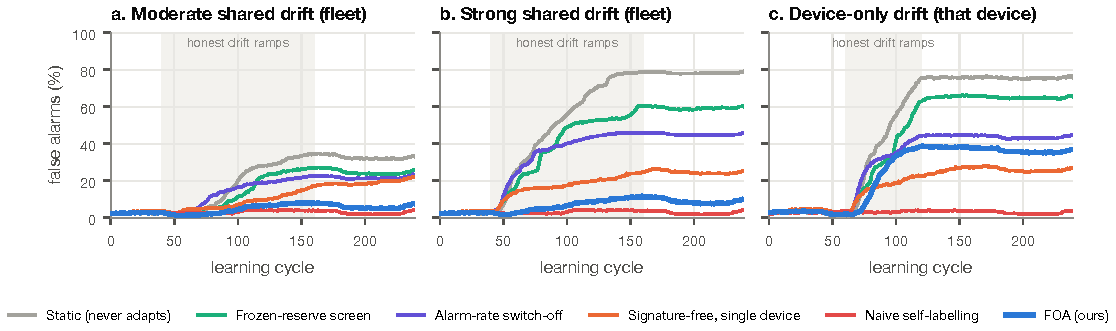
\includegraphics[width=\textwidth]{figures/fig_liveness.pdf}
\caption{False alarms with no attacker (10 held-out seeds). Shared drift (a, b) is followed by FOA through
the consensus; device-only drift (c) is admitted only at the residual rate $B$, the cost predicted by
Proposition~\ref{prop:frontier}.}
\label{fig:liveness}
\end{figure*}

\subsection{Safety: poisoning hidden inside drift}
With no drift (Table~\ref{tab:e2}), the signature-free local rule already resists most attackers
(\NoDriftAutoComp\ compromised against \NoDriftNaiveComp\ for naive learning), and FOA keeps that
(\NoDriftFOAComp). Drift is what breaks single-device defences: during a strong shared drift the
detector must move, and a poisoner moves with it. Table~\ref{tab:e3} and Figure~\ref{fig:headline}
show the result over \NRunsEThree\ runs. Against the classic boundary attacker FOA is compromised in
\FOABoundaryComp\ of runs at every share, against \AutoBoundaryComp\ for single-device adaptation (up to
\AutoBoundaryCompHigh\ at share 0.4). Over all three attacker types FOA is compromised in \FOAComp\ of
runs, single-device adaptation in \AutoComp, the alarm-rate switch-off in \KLComp\ and the frozen reserve
in \FrozenComp. Only TOA does better (\TOAComp), because it is handed the true attack signature, and it
pays for it with false alarms. FOA is the only rule in the lower-left corner of
Figure~\ref{fig:headline}b: few compromises \emph{and} few false alarms.

FOA is not unbreakable. A core-hiding attacker at share 0.4 compromises \FOACoreHigh\ of victims and a
mimicry attacker \FOAMimicHigh, almost all on the two Provision cameras, whose scan traffic is the
closest to benign among our victims. When FOA is compromised it takes longer: a median of \FOAMedTTC\
cycles after poisoning starts, against \AutoMedTTC\ for single-device adaptation. The bound of
Corollary~\ref{cor:ttc} was checked in every cycle of every attacked FOA run here and was violated
\BoundViolations\ times.

\begin{figure*}[t]
\centering
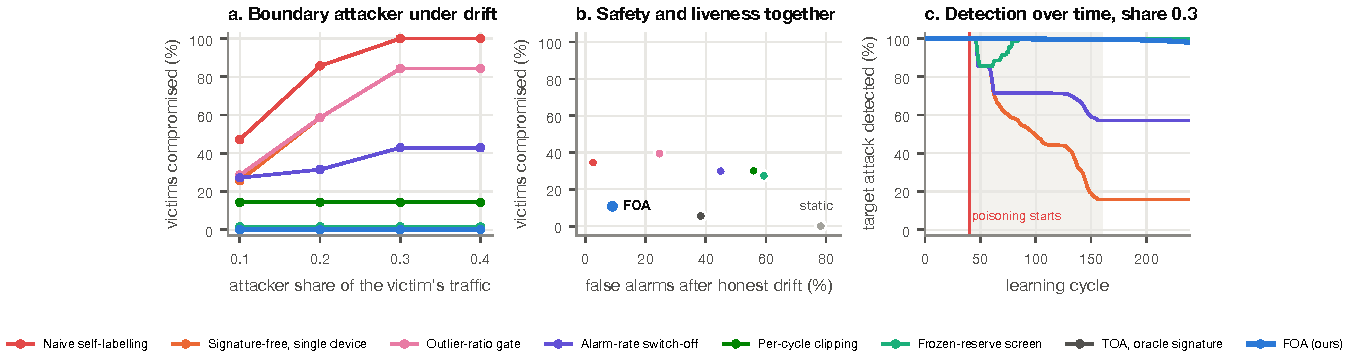
\includegraphics[width=\textwidth]{figures/fig_headline.pdf}
\caption{Poisoning hidden inside strong shared drift (7 victims, 10 held-out seeds, compromise counted
against an attacker-free twin). (a) Boundary attacker: FOA is never compromised. The outlier-ratio gate
never fires here and coincides with single-device adaptation. (b) Overall compromise against false
alarms after drift: FOA alone is low on both. (c) Mean detection of the target attack over time.}
\label{fig:headline}
\end{figure*}

% Generated by make_numbers.py. Do not edit.
\begin{table}[t]
\centering
\caption{False alarms (\%) after honest drift, no attacker. Shared drift: fleet mean; device-only: that device. 10 held-out seeds.}
\label{tab:liveness}
\small
\setlength{\tabcolsep}{4pt}
\begin{tabular}{@{}lrrr@{}}
\toprule
Rule & Moderate & Strong & Device-only \\
\midrule
Static & 32.7 & 78.3 & 75.6 \\
Naive & 2.6 & 2.6 & 2.6 \\
Single device & 18.9 & 24.6 & 26.0 \\
Clipping & 22.3 & 55.9 & 61.3 \\
Frozen reserve & 24.7 & 59.3 & 65.0 \\
Alarm switch-off & 21.7 & 45.0 & 43.5 \\
Outlier-ratio gate & 18.3 & 24.6 & 26.7 \\
TOA (oracle) & 28.5 & 38.3 & n/a \\
\textbf{FOA} & 6.0 & 9.0 & 36.1 \\
\bottomrule
\end{tabular}
\end{table}

\begin{table}[t]
\centering
\caption{Attack hidden in strong shared drift: victims compromised (\%, attack-attributable) by attacker type, averaged over shares 0.1 to 0.4, and false alarms after drift (\%). 7 victims, 10 held-out seeds.}
\label{tab:e3}
\small
\setlength{\tabcolsep}{4pt}
\begin{tabular}{@{}lrrrrrr@{}}
\toprule
Rule & Bound. & Core & Mimic. & All & FPR$_v$ & FPR$_{fl}$ \\
\midrule
Naive & 83 & 18 & 2 & 35 & 1.1 & 2.6 \\
Single device & 63 & 37 & 18 & 39 & 10.3 & 23.8 \\
Outlier-ratio gate & 64 & 37 & 18 & 39 & 10.5 & 23.8 \\
Alarm switch-off & 36 & 36 & 18 & 30 & 42.2 & 43.4 \\
Clipping & 14 & 46 & 30 & 30 & 51.0 & 54.0 \\
Frozen reserve & 1 & 52 & 28 & 27 & 66.6 & 57.2 \\
TOA (oracle) & 0 & 10 & 6 & 5 & 41.1 & 37.0 \\
\textbf{FOA} & 0 & 15 & 18 & 11 & 10.2 & 7.3 \\
\bottomrule
\end{tabular}
\end{table}

\begin{table}[t]
\centering
\caption{Poisoning with no drift: victims compromised (\%) by attacker type, averaged over shares 0.1 to 0.4.}
\label{tab:e2}
\small
\setlength{\tabcolsep}{4pt}
\begin{tabular}{@{}lrrrr@{}}
\toprule
Rule & Boundary & Core & Mimicry & All \\
\midrule
Naive & 86 & 21 & 1 & 36 \\
Single device & 0 & 15 & 7 & 7 \\
Alarm switch-off & 0 & 15 & 7 & 7 \\
Clipping & 0 & 14 & 1 & 5 \\
Frozen reserve & 0 & 9 & 3 & 4 \\
TOA (oracle) & 0 & 4 & 0 & 1 \\
\textbf{FOA} & 0 & 7 & 7 & 5 \\
\bottomrule
\end{tabular}
\end{table}

\begin{table}[t]
\centering
\caption{One knob: residual slope $B$ (alarm radii per cycle). Victims compromised under strong drift (boundary attacker, share 0.4, 4 victims) and false alarms after device-only drift (\%).}
\label{tab:sweep}
\small
\setlength{\tabcolsep}{4pt}
\begin{tabular}{@{}lrr@{}}
\toprule
$B$ & Compromised & Device-only FPR \\
\midrule
0.00125 & 0 & 55 \\
0.0025 & 0 & 43 \\
0.005 & 0 & 31 \\
0.01 & 50 & 29 \\
0.02 & 50 & 11 \\
0.04 & 75 & 16 \\
Single device & 75 & 20 \\
Alarm switch-off & n/a & 21 \\
Frozen reserve & n/a & 55 \\
Static & n/a & 65 \\
\bottomrule
\end{tabular}
\end{table}

\begin{table}[t]
\centering
\caption{Ablations under strong shared drift (3 victims, 10 seeds): victims compromised by a boundary attacker at share 0.3 (\%), fleet false alarms after drift (\%), and false alarms on a device with its own drift on top of the shared one (\%).}
\label{tab:ablation}
\small
\setlength{\tabcolsep}{4pt}
\begin{tabular}{@{}lrrr@{}}
\toprule
Variant & Comp. & FPR$_{fl}$ & FPR$_{own}$ \\
\midrule
FOA (default) & 0 & 7.0 & 90 \\
mean instead of geometric median & 0 & 5.9 & 74 \\
coordinate-wise median & 0 & 6.9 & 90 \\
mean-based agreement & 0 & 13.8 & 90 \\
no agreement ($\lambda=1$) & 0 & 11.5 & 90 \\
no significance ($w=1$) & 0 & 10.1 & 90 \\
no common budget & 0 & 7.0 & 90 \\
2$\times$ wider spread budget & 33 & 10.0 & 90 \\
joint centre+spread budget & 33 & 15.2 & 42 \\
no residual budget & 67 & 23.4 & 57 \\
discard residual (CIoTA-like) & 0 & 53.6 & 100 \\
no peers (budget only) & 0 & 43.0 & 100 \\
2 diverse peers & 7 & 9.7 & 80 \\
3 diverse peers & 3 & 8.6 & 80 \\
3 random peers & 3 & 8.1 & 81 \\
all peers & 0 & 7.2 & 90 \\
\bottomrule
\end{tabular}
\end{table}



\subsection{Monoculture botnets: why the peers must be diverse}
The twelve-device fleet has three instances each of four models. A botnet infects $k$ of the three
SimpleHome XCS7-1003 cameras and poisons all of them together during strong drift
(Figure~\ref{fig:monoculture}; without drift no rule was compromised). Same-model consensus, as in CIoTA~\cite{ciota}, works while the
infected cameras are a minority of their group: with one of three infected it is compromised in
\MonoCiotaOne\ of runs. Once two or three of the three are infected, the consensus \emph{is} the botnet,
and it is compromised in \MonoCiotaThree\ of runs; FOA restricted to same-model peers fails the same way
(\MonoSameThree). FOA with vulnerability-diverse peers is compromised in \MonoFOAThree\ of runs at every
$k$, as is FOA listening to all peers, because one exploit reaches at most three of eleven peers. This
is the head-to-head that separates FOA from same-model consensus. In this fleet, diversity has a cost:
a device whose only diverse peers are three other models gets a coarser consensus and higher false
alarms than one listening to all peers, so in practice a peer group should be as large as possible
subject to no single vulnerability class holding half of it.

\begin{figure}[t]
\centering
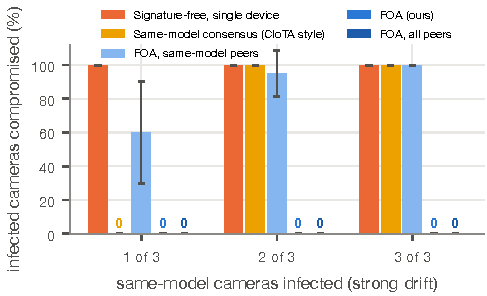
\includegraphics[width=\columnwidth]{figures/fig_monoculture.pdf}
\caption{Monoculture botnet: $k$ of three same-model cameras are infected and poisoned together.
Same-model consensus fails as soon as the infected cameras are a majority of their model; FOA with
diverse peers does not.}
\label{fig:monoculture}
\end{figure}

\subsection{The freeze attack}
An attacker sends loud decoy traffic (real attack packets, pushed out to twice the alarm radius) to one
device from cycle 40 to 100, while strong honest drift runs from cycle 40 to 160, and then leaves
(Figure~\ref{fig:freeze}). Decoys are never learned from by any rule; their only possible effect is on a
stop-learning gate. The alarm-rate switch-off closes as soon as decoys arrive, honest drift moves on
without it, and when the attacker leaves the alarm rate stays high because the traffic has drifted
away: the gate never reopens and the device ends at \KLFrozenFPR\ false alarms, against \KLCleanFPR\
for the same gate without the attacker, at every decoy share from 5\% upward. Not every gate freezes:
the outlier-ratio gate compares the alarm rate with its own moving average, which rises with the decoys,
so it reopened and ended where it would have without the attacker (\ORFrozenFPR); the frozen reserve has
no gate to trip but suffers from the drift itself. FOA's trajectory is unchanged (\FOAFreezeFPR\ with the attacker,
\FOAFreezeClean\ without), exactly as Proposition~\ref{prop:freeze} states; our unit tests check that the
two trajectories are bit-for-bit identical. This holds in simulation, where decoys are separate samples;
on our boards, whose features summarise all incoming packets together, a decoy flood would shift every
sample (Section~\ref{sec:theory}).

\begin{figure*}[t]
\centering
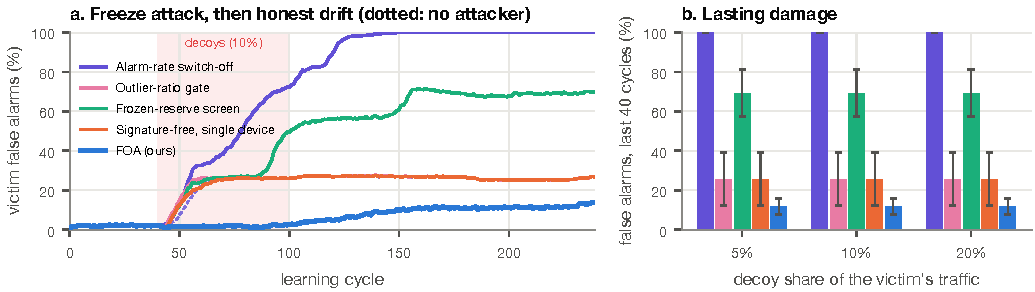
\includegraphics[width=\textwidth]{figures/fig_freeze.pdf}
\caption{Freeze attack. (a) False alarms on the targeted device; decoys from cycle 40 to 100 (10\% share),
honest drift from 40 to 160. Dotted: same rule, no attacker. (b) False alarms over the last 40 cycles
by decoy share.}
\label{fig:freeze}
\end{figure*}

\subsection{Attacks on the gossip}
\textbf{Byzantine peers.} We give the attacker full control, keys included, of $f$ of a victim's seven or
eight diverse peers, during strong drift, for five victims (Figure~\ref{fig:gossip}a). Four of seven peers is past the breakdown point of
Theorem~\ref{thm:byz} and four of eight is at it, so $f=4$ lies outside the theorem. On their own,
Byzantine peers compromised no victim at any $f$ up to four (\ByzAloneMax): the victim's own traffic does
not back what they send, and its agreement $\lambda$ stays low. Combined with a traffic poisoner on the
victim, they erode FOA's protection gradually: \ByzTZ, \ByzTO, \ByzTH\ of victims compromised with
0, 1 and 3 Byzantine peers and \ByzTF\ with four, against \ByzAuto\ for single-device adaptation under
the poisoner alone. The victims that fall are the three closest to their benign traffic (1.5 to 1.9 alarm
radii); the two with larger margins were never compromised. Tracing the runs, the extra help travels
mostly through the common spread channel: Byzantine frames report spread growth, the poisoned victim's
own proposals agree, and a small extra inflation tips a borderline victim. We tried two repairs on the
development seeds (letting the device's own median shift choose the common direction, with significance
judged from its own noise; and a tighter common spread budget); neither changed this outcome, so we
report it as a limit.
\textbf{Keyless attackers.} Twelve forged frames per cycle plus replays of the previous cycle's frames
had no effect (\SybilFOA\ compromised; every forged and replayed frame was rejected). With
authentication switched off, the same attacker compromised the victim in \SybilNoHMAC\ of runs.
\textbf{Lossy radio.} Losing up to 70\% of frames changed little (fleet false alarms \LossNoneFPR\
with no loss, \LossHalfFPR\ at 50\%); at 90\% most cycles have fewer than two peers, FOA falls back to
its residual budget and false alarms rise.

\begin{figure*}[t]
\centering
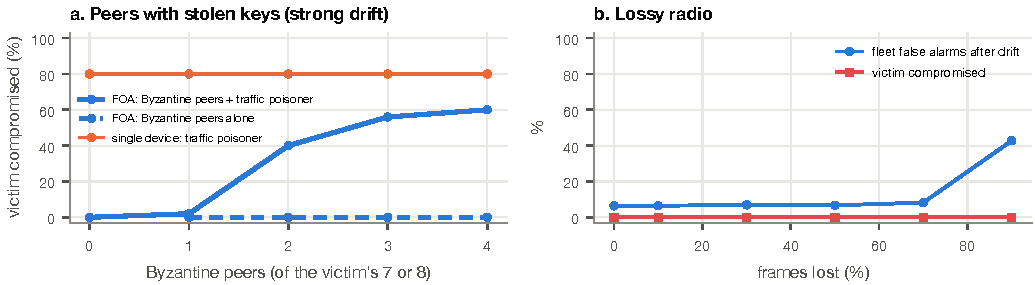
\includegraphics[width=0.8\textwidth]{figures/fig_gossip.pdf}
\caption{Attacks on the gossip. (a) Byzantine peers with valid keys, alone and together with a traffic poisoner on the victim (strong drift, 5 victims, 10 held-out seeds). (b) Frame loss.}
\label{fig:gossip}
\end{figure*}

\subsection{One knob: the residual rate}\label{sec:frontier}
Table~\ref{tab:sweep} sweeps $B$. With $B\le$\SweepSafeMaxB\ alarm radii per cycle no victim was
compromised; larger $B$ admits the attacker faster (\SweepCompHigh\ compromised at $B=0.04$). In
exchange, a device's own drift is followed faster: false alarms after device-only drift fall from
\SweepIdioLow\ at the smallest $B$ to \SweepIdioHigh\ at $B=0.02$. No setting is free, as
Proposition~\ref{prop:frontier} says; the bound of Corollary~\ref{cor:ttc} held in every run of the
sweep (\SweepViol\ violations). Figure~\ref{fig:theory} repeats the sweep on a synthetic fleet with known
geometry and checks the Byzantine lemma numerically.

\begin{figure*}[t]
\centering
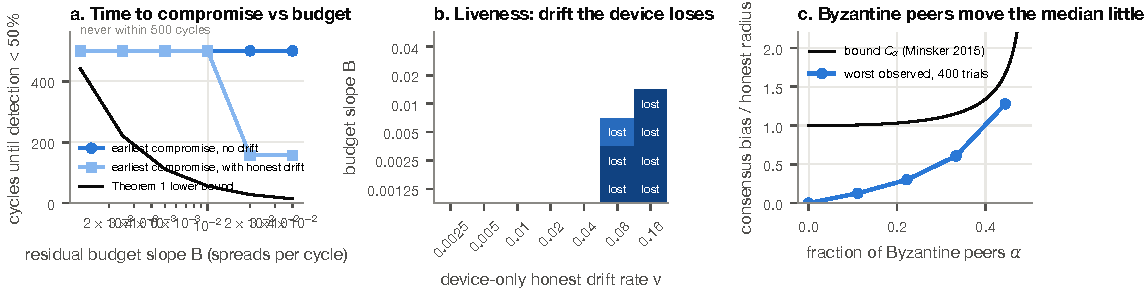
\includegraphics[width=\textwidth]{figures/fig_theory.pdf}
\caption{Theory checks on a synthetic fleet with known geometry. (a) Earliest compromise against the
budget slope, with the closed-form lower bound of Corollary~\ref{cor:ttc}. (b) Device-only drift rates
that a device loses, for each budget slope. (c) Worst observed consensus bias with $f$ Byzantine peers
against Lemma~\ref{lem:gm}.}
\label{fig:theory}
\end{figure*}

\subsection{Ablations and adaptive attackers}\label{sec:ablation}
Table~\ref{tab:ablation} removes one piece at a time. Discarding the residual instead of rationing it
(the CIoTA choice applied to diverse peers) leaves devices unable to follow anything their peers do not
share: fleet false alarms rise to \AblDiscardFPR. Removing the peers (budget only) gives
\AblNoPeersFPR. Removing the residual budget gives back the attack (\AblFullComp\ compromised). Measuring
agreement with a mean instead of a median roughly doubles false alarms (\AblMeanLamFPR\ against
\AblFOAFPR), because an attacker can then cancel the victim's agreement and stall it. A wider spread
budget or a joint centre-and-spread budget lets attackers through: inflating the spread is the cheapest
way to make an attack fit. When a device has its own large drift on top of the shared one, almost every
variant loses that device (false alarms of 74 to 100\%); only the variants with more room (no residual
budget, or one joint budget) partly keep up, and both are poisoned. Removing the residual budget is also
the only change that ever violated the bound of Corollary~\ref{cor:ttc} (4 runs), as it should. Among
adaptive attackers (strong drift, share 0.3, three victims), pulsing compromised no one under either
rule; FOA cut the core-hiding attacker from 33\% to 10\%; and multi-direction, consensus-aligned and
mimicry attackers each compromised one of the three victims (33\%) under both FOA and single-device
adaptation, so FOA did not help against them on that victim.

\subsection{A four-node fleet}
Small testbeds have few peers. Simulating a fleet of four vendors (Danmini, Ecobee, Provision PT-838,
SimpleHome XCS7-1003) with strong drift and a boundary attacker at share 0.3: FOA \FourCompFOA\
compromised with \FourFPRFOA\ fleet false alarms; single-device adaptation \FourCompAuto\ and
\FourFPRAuto; alarm-rate switch-off \FourCompKL\ and \FourFPRKL; frozen reserve \FourCompFrozen\ and
\FourFPRFrozen. Three peers are enough for the consensus to work. Joining devices were never
compromised in our join experiment (\JoinComp), with or without the warm start.

\input{eval_cesnet.tex}


\subsection{Cost on an ESP32}\label{sec:cost}

FOA's on-device part is about 500 lines of portable C99 with no heap: the detector, the signature-free
proposal with the median agreement projection, ten Weiszfeld iterations, the FOA step, the 92-byte frame
and HMAC-SHA256. Table~\ref{tab:cost} summarises the checks made without hardware; Section~\ref{sec:hw} reports measurements on boards.

\textbf{Equivalence.} On 480 recorded cycles from three synthetic fleets (one with 85\% frame loss, so
130 cycles had fewer than two peers), the C proposal matches the Python reference to a worst relative
error of $5.4\times10^{-4}$ (float32 against float64) and the C FOA step to $6\times10^{-5}$, with zero
mismatches. Frames packed in C are byte-identical to Python's; all 23{,}040 single-bit flips, wrong keys
and stale cycle numbers are rejected; HMAC-SHA256 passes RFC 4231 test case 2.

\textbf{Footprint.} Compiled for the ESP32 (Arduino-ESP32 core 3.3.12) the node firmware uses
915{,}504 bytes of flash and 69{,}216 bytes of static RAM; the same Wi-Fi, UDP and ESP-NOW code without
FOA uses 893{,}284 and 48{,}928. FOA therefore costs about 22\,KB of flash and 20\,KB of static RAM, of
which 13\,KB is the batch of 200 sixteen-dimensional samples; calibration borrows about 80\,KB of heap once and
frees it. The detector and FOA state are 452 bytes.

\textbf{Time and energy (estimates).} On the laptop one proposal over 200 points takes 5\,$\mu$s, one FOA
step with 8 peers 0.7\,$\mu$s and one frame signature 1.2\,$\mu$s. The step is about $3{\times}10^4$
floating-point operations plus a few hundred square roots; at 240\,MHz and a conservative ten cycles per
operation this is about 2\,ms per learning cycle, against a cycle length of 10\,s. One 92-byte ESP-NOW
broadcast per cycle is about 1\,ms of airtime. These are estimates; the firmware logs the measured time
of every stage and the INA219 monitor gives energy per cycle on the testbed.

\begin{table}[t]
\centering
\caption{FOA on the ESP32: verified before hardware, and estimated}
\label{tab:cost}
\small
\begin{tabular}{@{}lr@{}}
\toprule
C vs Python, 480 cycles & 0 mismatches \\
Tampered frames accepted & 0 of 23{,}104 \\
Added flash / static RAM & 22\,KB / 20\,KB \\
State per device & 452 B \\
Gossip per device per cycle & one 92 B frame \\
Compute per cycle (est.) & $\approx$2\,ms at 240\,MHz \\
\bottomrule
\end{tabular}
\end{table}


\subsection{All rules across attacks and conditions}\label{sec:compare}

Figure~\ref{fig:compare} gathers the compromise results for every signature-free rule in four settings:
strong shared drift with all attacker types, the classic boundary poisoner, poison hidden in the clean
core, and a one-model botnet with two of three cameras infected. Table~\ref{tab:compare} gives the
numbers and the false alarms that each rule pays.

\begin{figure*}[t]
\centering
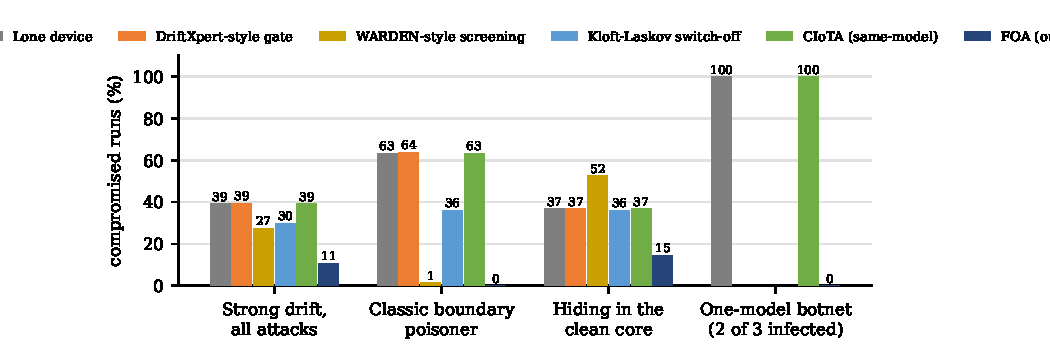
\includegraphics[width=\textwidth]{figures/fig_compare.pdf}
\caption{Compromised runs (\%) for each rule. Drift settings: 7 victims, 4 attacker shares, 10 held-out
seeds (840 runs per rule). Botnet: strong drift, 2 of 3 same-model cameras infected. Missing bars were not
run in that setting. CIoTA-style equals the lone device under drift because the nine-device fleet has
no three devices of one model, so it has no one to vote with.}\label{fig:compare}
\end{figure*}

\begin{figure*}[t]
\centering
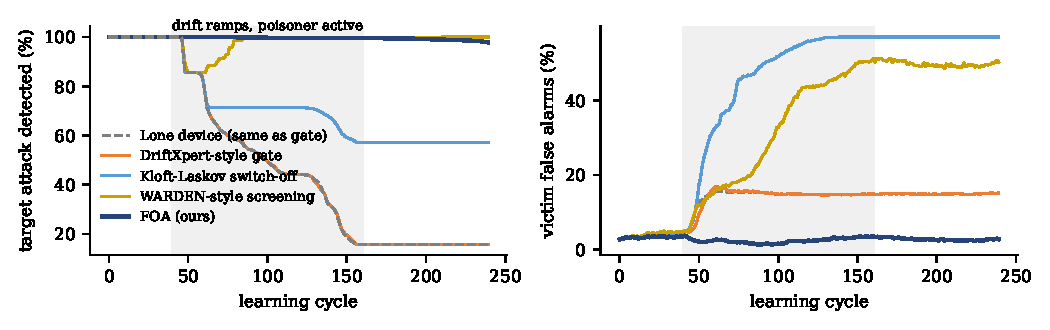
\includegraphics[width=\textwidth]{figures/fig_frog.pdf}
\caption{The boiling frog in action: classic boundary poisoner at share 0.3 during strong shared drift
(shaded: drift ramps and the poisoner is active), mean over 7 victims and 10 held-out seeds. Left:
share of the target attack still detected. Right: victim false alarms. The lone device (dashed) and the
outlier-ratio gate coincide.}\label{fig:frog}
\end{figure*}

\begin{table}[t]
\caption{Compromised runs (\%) by setting, and fleet false alarms after strong honest drift (\%, Table~\ref{tab:liveness}). Lower is better. -- : not run}\label{tab:compare}
\centering\footnotesize\setlength{\tabcolsep}{3.2pt}
\begin{tabular}{@{}lrrrrr@{}}
\toprule
Rule & All & Bound. & Core & Botnet & FPR \\
\midrule
Naive & 35 & 83 & 18 & -- & 2.6 \\
Single device & 39 & 63 & 37 & 100 & 24.6 \\
Outlier-ratio gate & 39 & 64 & 37 & -- & 24.6 \\
Alarm switch-off & 30 & 36 & 36 & -- & 45.0 \\
Clipping & 30 & 14 & 46 & -- & 55.9 \\
Frozen reserve & 27 & 1 & 52 & -- & 59.3 \\
CIoTA-style & 39 & 63 & 37 & 100 & -- \\
\textbf{FOA} & \textbf{11} & \textbf{0} & \textbf{15} & \textbf{0} & \textbf{9.0} \\
\midrule
TOA (oracle) & 5 & 0 & 10 & -- & 38.3 \\
\bottomrule
\end{tabular}
\end{table}

\textbf{Reading the comparison.} Among rules that do not know the attack in advance, FOA has the lowest
compromise rate overall (11\% against 27\% to 39\%), is never compromised by the boundary poisoner or by
the one-model botnet, and has the lowest rate for poison hidden in the clean core (15\%). The defences
that come closest on one attack pay elsewhere: the frozen reserve stops the boundary poisoner (1\%) but
is compromised in 52\% of core runs and raises 59\% false alarms; the alarm switch-off and clipping trade
safety for 45\% to 56\% false alarms. Only TOA is safer, and only because it is given the attack's
signature. Under the mimicry attacker, who imitates the shared drift, FOA (18\%) is not better than a lone
device (18\%) and the naive rule (2\%) does best (Table~\ref{tab:e3}); this is the case
Proposition~\ref{prop:frontier} predicts, because that attacker hides inside change the neighbours do see.

\begin{table}[t]
\caption{Outcome of each hypothesis}\label{tab:hyp}
\centering\footnotesize
\begin{tabular}{@{}p{1.25cm}p{4.7cm}p{1.45cm}@{}}
\toprule
Hypothesis & Evidence & Outcome \\
\midrule
H1 safety & 10.8\% compromised vs 39.2\% (single device) and 27\% to 30\% (gated); 9.4\% vs 43.1\% with the floor & Supported \\
H2 tracking & With the floor, 2.5\% fleet false alarms after strong drift vs 0.8\% for a single device & Supported \\
H3 cost & 1.2 to 1.9\,ms to combine, 92-byte frames, extra energy below sensor resolution on ESP8266 & Supported \\
H4 robustness & One-model botnet 0\% vs 100\% (same-model voting); decoys leave FOA's trajectory unchanged & Supported \\
\bottomrule
\end{tabular}
\end{table}

\section{On Real Boards: a Failure and a Fix}\label{sec:hw}

\subsection{Testbed}
We ran FOA on three ESP8266 NodeMCU boards on a phone hotspot, gossiping over ESP-NOW, with an INA226
sensor in the supply line of one board. The firmware reuses the portable C core. The feature basis is a
placeholder (not yet fitted on testbed traffic) and the keys are development keys. Two runs of about 20
minutes were logged; no attack was run on the boards.

\begin{table}[t]
\centering
\caption{Three-board testbed (medians; run in which all boards started together)}
\label{tab:hw}
\small
\begin{tabular}{@{}lr@{}}
\toprule
Cycles hearing both neighbours & 97 to 100\% \\
Update proposal / FOA step & 11.2\,ms / 1.6\,ms \\
Sign one frame / verify two & 0.60\,ms / 0.95\,ms \\
Learning cycle period & 7.77\,s \\
Board power (second run) & 365\,mW at 5.04\,V \\
Energy per cycle, whole board & 2.84\,J \\
\bottomrule
\end{tabular}
\end{table}

No extra energy for a learning cycle was detectable with the sensor sampling every 40\,ms: power in the
0.6\,s learning window was in fact $4.2\pm0.1$\,mJ \emph{below} normal running, plausibly because the
board mostly waits for frames then. About 19\,ms of computing per cycle at full board power would be
about 7\,mJ; this is an estimate. Deployment also exposed defects that simulation had not: frames were
rejected because boards boot at different times (now each sender's cycle number must only increase), and
calibration ran before the damped statistics had settled (now preceded by a warm-up).

\subsection{The collapse}
When all three boards started together, every detector's spread shrank to under 2\% of its calibrated
value within 20 minutes and false alarms reached about 90\% (Figure~\ref{fig:hw}). The board traffic is
highly repetitive. The core-only rule may shrink the spread freely while growth is gated by outer-ring
support, a one-way ratchet; identical boards agree on the shrink, and FOA applies it as common change.
In a second run, two restarted boards beside an already collapsed one levelled off near 54\%, which is
consistent with this account but does not prove it; the placeholder basis may also contribute. A
simulation of repetitive traffic with no attacker reproduces the collapse.

\begin{figure*}[t]
\centering
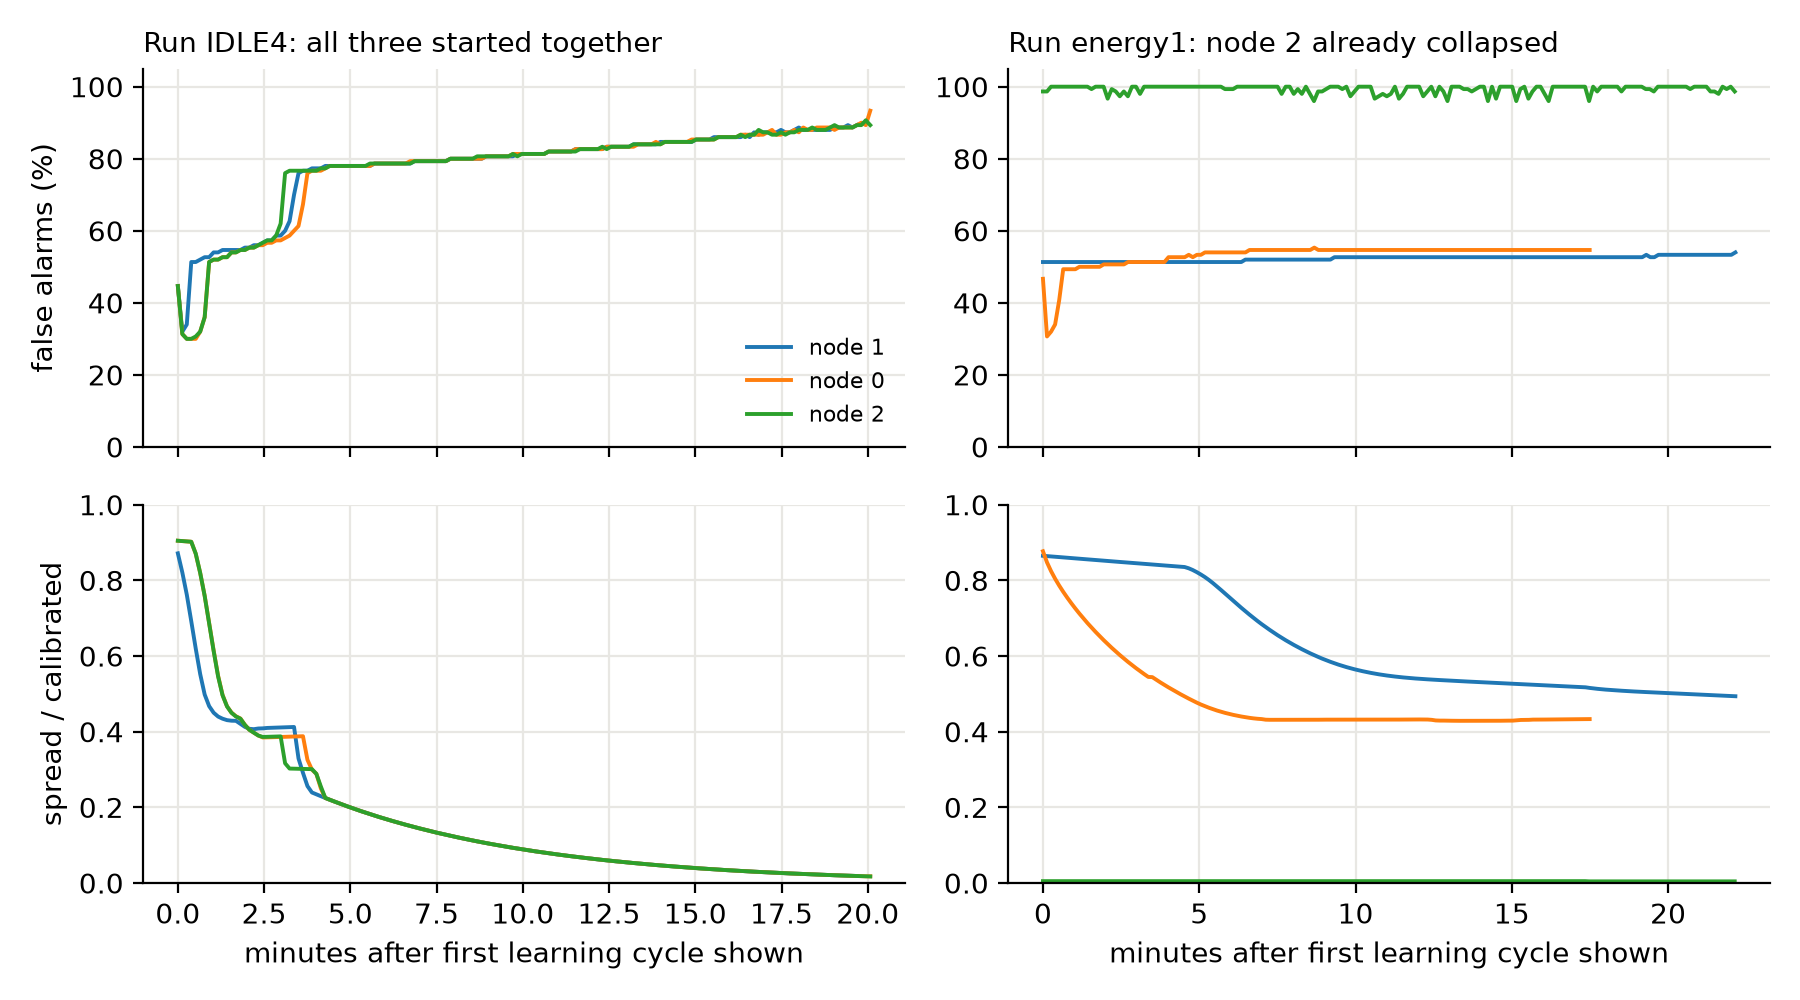
\includegraphics[width=0.85\textwidth]{figures/hardware_results.png}
\caption{The two testbed runs: false alarms and spread relative to calibration. Left: all boards started
together and collapsed. Right: one board had already collapsed; the two restarted boards levelled off.}
\label{fig:hw}
\end{figure*}

\subsection{The coverage floor}\label{sec:floor}
The fix is one rule: the spread may never shrink below its calibrated value, $s_i(t)\ge s_i^0$. It only
moves increments toward zero, so both budgets and Theorem~\ref{thm:contain} still hold (checked: no bound
violation in 1{,}710 attacked runs with the floor). We chose it on development seeds and evaluated it on
held-out seeds (Table~\ref{tab:floor}); the C core with the floor matches the reference.

\begin{table}[t]
\centering
\caption{The coverage floor on held-out seeds 2 to 11: false alarms (\%) after moderate, strong and device-only drift, and victims compromised (\%) without drift, by the boundary attacker under strong drift, and by all attackers under strong drift.}
\label{tab:floor}
\small
\setlength{\tabcolsep}{3pt}
\begin{tabular}{@{}lrrrrrr@{}}
\toprule
Rule & Mod. & Strong & Own & None & Bound. & All \\
\midrule
Single device & 18.9 & 24.6 & 20.3 & 7.4 & 63.2 & 39.2 \\
Single device + floor & 0.9 & 0.8 & 0.9 & 7.6 & 75.4 & 43.1 \\
FOA & 6.0 & 9.0 & 28.2 & 4.6 & 0.0 & 10.8 \\
\textbf{FOA + floor} & 1.4 & 2.5 & 24.6 & 4.3 & 0.0 & 9.4 \\
\bottomrule
\end{tabular}
\end{table}


On repetitive traffic (20 held-out runs) the floor cuts mean false alarms from 13.2\% to 1.5\% and the
worst run from 75\% to 5.4\%. It also changes the reading of Section~\ref{sec:eval}. \textbf{Most of
single-device adaptation's false alarms were caused by the same ratchet}: with the floor a single device
reaches \FlAutoFStrongFPR\ under strong drift, lower than FOA with the floor (\FlFOAFStrongFPR), and it
also follows its own drift far better (\FlAutoFIdioFPR\ against \FlFOAFIdioFPR). FOA's earlier
false-alarm advantage over a single device therefore does not survive. What survives, and is the reason
to use FOA, is safety under drift: with the floor in both, FOA is compromised in \FlFOAFCompStrong\ of
runs against \FlAutoFCompStrong\ for a single device, never by the boundary attacker against
\FlAutoFCompBound, and it still withstands the monoculture botnet that defeats a single device in every
run. The floored rule has not yet been run on the boards.

\section{The Research Journey}\label{sec:journey}

FOA was not our first design. Figure~\ref{fig:journey} traces how each idea answered the weakness of the
one before, and what each step taught us.

\begin{figure*}[t]
\centering
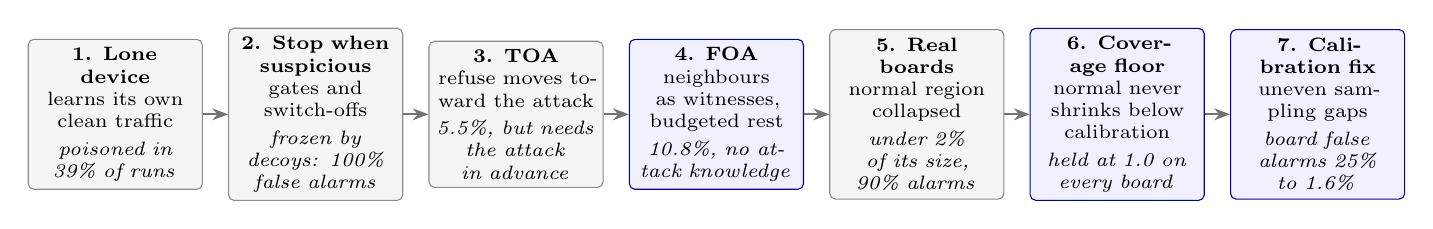
\begin{tikzpicture}[node distance=0.32cm,
  st/.style={draw=black!45, rounded corners=2pt, fill=black!4, text width=2.0cm, minimum height=1.55cm, align=center, font=\scriptsize, inner sep=3pt},
  hi/.style={st, draw=blue!70!black, fill=blue!6},
  ar/.style={-{Stealth[length=2mm]}, black!55, thick}]
\node[st] (a) {\textbf{1. Lone device}\\ learns its own clean traffic\\[2pt] \textit{poisoned in 39\% of runs}};
\node[st, right=of a] (b) {\textbf{2. Stop when suspicious}\\ gates and switch-offs\\[2pt] \textit{frozen by decoys: 100\% false alarms}};
\node[st, right=of b] (c) {\textbf{3. TOA}\\ refuse moves toward the attack\\[2pt] \textit{5.5\%, but needs the attack in advance}};
\node[hi, right=of c] (d) {\textbf{4. FOA}\\ neighbours as witnesses, budgeted rest\\[2pt] \textit{10.8\%, no attack knowledge}};
\node[st, right=of d] (e) {\textbf{5. Real boards}\\ normal region collapsed\\[2pt] \textit{under 2\% of its size, 90\% alarms}};
\node[hi, right=of e] (f) {\textbf{6. Coverage floor}\\ normal never shrinks below calibration\\[2pt] \textit{held at 1.0 on every board}};
\node[hi, right=of f] (g) {\textbf{7. Calibration fix}\\ uneven sampling gaps\\[2pt] \textit{board false alarms 25\% to 1.6\%}};
\foreach \x/\y in {a/b,b/c,c/d,d/e,e/f,f/g} \draw[ar] (\x) -- (\y);
\end{tikzpicture}
\caption{How the design evolved. Each step fixed the weakness the previous one exposed.}\label{fig:journey}
\end{figure*}

\textbf{From a lone device to gates.} Self-labelled learning on one device is the natural starting point,
and it is exactly what the boiling frog exploits. Stopping learning on suspicion protects against it but
introduces the freeze attack (Section~\ref{sec:eval}): five percent decoys locked the alarm switch-off at
\KLFrozenFPR\ false alarms.

\textbf{From TOA to FOA.} Our first method, Threat-Orthogonal Adaptation, refused movement toward the
known attack direction. It is very safe (5.5\% compromised) but needs the attack's signature in advance,
which a deployed device never has, and it raised 38\% false alarms. FOA replaces that oracle knowledge
with a witness a device does have: its neighbours.

\textbf{From simulation to boards.} On three ESP8266 boards the detectors shrank their normal regions in
agreement until almost everything alarmed (Section~\ref{sec:hw}). The cause, a guard on growth with none
on shrinking, was reproduced in simulation with no attacker. The coverage floor fixed it, held on every
board, and corrected our own claim: FOA's lasting advantage is safety under drift. A second fault,
calibration sampling in step with the 200\,ms telemetry, explained the remaining false alarms; uneven
sampling gaps brought them to 1.5\% to 1.7\%.

\textbf{Lessons.} (i) A defence that can stop learning can be made to stop. (ii) A second witness beats
a stronger single witness. (iii) Guard both directions of change, not only the one an attacker uses.
(iv) Test on hardware early: the boards found two faults that thousands of simulated runs did not.

\section{Related Work}\label{sec:related}

\textbf{Poisoning self-updating detectors.} Rubinstein et al.\ showed that a network anomaly detector
that retrains on its own traffic can be walked toward an attack by slowly increasing chaff, the
boiling-frog attack, and defended it with robust PCA on a server~\cite{antidote}. Kloft and Laskov
analysed exactly our detector, the online centroid, and showed that the attacker's share of the training
traffic bounds how far it can be moved; they also proposed switching learning off when the alarm rate
rises~\cite{kloft}. Poisoning of test-time adaptation~\cite{su2025tta}, of on-device learning on
microcontroller-class hardware~\cite{sensors2024}, and of rapid-response adaptation
pipelines~\cite{rapidpoison} shows the problem is current. A 2026 survey of on-device learning in
TinyML does not discuss security or poisoning~\cite{tinymlsurvey}. FOA targets this
gap with a per-device detector that adapts on the device.

\textbf{Adaptive intrusion detection and its gates.} Kitsune made online, per-packet anomaly
detection practical but stops learning after training~\cite{kitsune}. Later adaptive detectors decide
\emph{when} to learn: OWAD detects normality shift and adapts after a test~\cite{owad}; DriftXpert
triggers retraining when an outlier ratio rises~\cite{driftxpert}; RTTAD adapts in rounds on the test
samples it is confident about, both normal and anomalous, and ends when too few such samples
remain~\cite{rttad}; a continual-learning analysis of poisoning proposes rolling back
when the score spikes~\cite{clpoison}; ACORN-IDS and CND-IDS continue learning from normal-only
streams~\cite{acorn,cndids}. Each decides from a traffic statistic when to learn, and several stop
learning when traffic looks suspicious. Our freeze experiments show that an attacker who can make such
a stop condition true with loud traffic can turn honest drift into a
lasting flood of false alarms. Korycki and Krawczyk discussed attacks that impair adaptation in data
streams~\cite{korycki}; we found no prior evaluation of this freeze effect on the gating rules of
adaptive intrusion detectors.

\textbf{Limits of a single stream.} Recent theory (all 2026 preprints) shows that one label-free score
stream cannot separate honest drift from slow contamination (WARDEN~\cite{warden}), that regularised
continual learners cannot converge under frequent shifted poison~\cite{clpoison}, and that a single
statistic forces a choice between accepting injected changes and rejecting genuine ones
(CAPTURE~\cite{capture}). A further preprint frames self-calibration as an evidence budget with blind
sets~\cite{selfcal}; we have read only its abstract. FOA does not contradict these results; it changes
the observation model by adding peers, and Proposition~\ref{prop:frontier} states what remains impossible.

\textbf{Collaborative detection and robust aggregation.} The closest prior work is
CIoTA~\cite{ciota}: devices of the same model train models collaboratively and accept an update only
when the group agrees, discarding the rest. FOA differs in three ways: peers are chosen to be
vulnerability-\emph{diverse}, so a monoculture botnet cannot manufacture consensus; the remainder is
\emph{rationed} through a budget rather than discarded, which keeps a device able to follow its own
changes; and the guarantee is a bound on movement and time to compromise, not agreement. Byzantine-robust
aggregation (Krum~\cite{krum}, the geometric median~\cite{lopuhaa,minsker}) protects a shared model in
federated learning; FOA uses the geometric median only to estimate the common component of per-device
updates, and keeps every device's own detector.

Structurally, FOA is closest to consensus with a bounded local term. In the saturated innovation update
of Chen, Kar and Moura, sensors combine a consensus step with a norm-limited local innovation and still
estimate a fixed parameter when fewer than half of them are attacked~\cite{siu}; BALANCE accepts a
neighbour's model only within a distance that shrinks over time~\cite{balance}; ClippedGossip clips
neighbours' updates~\cite{clippedgossip}. These target a fixed optimum with a tolerance that shrinks,
which would reject honest drift that arrives late; FOA tracks a moving normal with a residual allowance
that grows. We have not compared against them experimentally. The intuition is not new in practice either: a
Darktrace patent describes continually updated per-entity models that compare each entity with its own
history and with its peers', so that compromised entities, which behave unlike their peers, are not
learned as normal~\cite{darktrace}. What FOA adds is a specific rule with a stated bound on how fast one device
can be moved, the freeze analysis, and an implementation on microcontrollers.

\section{Discussion and Limitations}\label{sec:discussion}

\textbf{What is real and what is modelled.} The benign and attack traffic are real N-BaIoT
captures~\cite{nbaiot}, and the C implementation is real: compiled for the ESP32 and run on three ESP8266 boards. Three things are
ours and synthetic: the concurrency of the fleet (the nine devices were captured separately), the honest
drift (physically modelled transforms of the Kitsune statistics, not a recorded network change), and the
poisoner (crafted feature vectors, not packets). A public intrusion dataset with documented concept
drift did not exist when the 2025 survey of intrusion datasets was written~\cite{nidsurvey}, which is
why the drift is injected; the testbed's real common-mode drift is the next step.

\textbf{The frontier cannot be escaped, only placed.} Proposition~\ref{prop:frontier} is a limit on
every rule, not a weakness of FOA: a device's own drift and an attack on that device look the same to
everyone else. FOA's contribution is to move all drift the peers can vouch for out of that dilemma and
to make the remaining trade-off one explicit number, $B$. A deployment that expects frequent device-only
changes (firmware updates) can raise $B$ for a bounded window when the update is signed and announced, as
licensed-update schemes do; we leave that to future work.

\textbf{When the fleet is the attacker.} If one exploit compromises a majority of a device's peer group,
or a gateway rewrites everyone's traffic, consensus carries the attack. Vulnerability-diverse peers make
the first harder, not impossible: N-BaIoT itself shows that one credential-guessing botnet (BASHLITE)
infected all nine devices~\cite{nbaiot}. FOA then degrades to its residual budget and common-channel
budget, which still bound the rate of movement (Theorem~\ref{thm:byz}), but not to safety.

\textbf{Limits we measured.} Three results are against FOA and we report them as such. Byzantine
peers cannot compromise a device on their own, but together with a traffic poisoner they help it: with
three of seven peers controlled, about half of the victims fell during strong drift, all of them victims
whose attack traffic sits close to their benign traffic. A device with a large drift of its own on
top of the shared one is lost by FOA (and by every budgeted variant), while single-device adaptation
keeps it. Core-hiding and mimicry attackers at share 0.4 still compromised about a third of victims,
mostly the two cameras whose scan traffic is closest to benign.

\textbf{Spread is the attacker's lever.} In the compromised runs we traced, the successful attacks
inflated the spread rather than dragging the centre, the radius attack Kloft and Laskov warned
about~\cite{kloft}. FOA's spread budget is what holds it, and it is the parameter we would tune first.

\textbf{Where FOA fits.} For a single-purpose device, an allow-list of the endpoints its maker intends,
as in Manufacturer Usage Descriptions~\cite{mud}, cannot be poisoned at all and catches scanning and
flooding without learning; anomaly detection, and so FOA, matters where normal behaviour is too varied
or changes too often to list. An infected device can also stop its own detector, as Mirai kills
competing processes~\cite{mirai}, so a deployment would more naturally run one FOA detector per device
on a gateway or edge box, with peers drawn from other devices and sites, and with someone to act on its
alarms. Our false-alarm rates are per sample; an operator needs alerts per device per day, which we did
not evaluate. The pattern itself, per-entity baselines that must follow shared change but not one
entity's slow manipulation, is wider than IoT, and peer comparison is already used in commercial
network detection~\cite{darktrace}.

\textbf{Hardware.} Section~\ref{sec:hw} reports three ESP8266 boards. The floor now holds on them, but
attack and freeze tests on hardware, a testbed-fitted feature basis, repeated runs and recovery from
abrupt change remain to be done. The board firmware summarises all incoming packets together, so on the
boards an attacker's traffic shifts every sample instead of adding separate ones; statistics kept per
source would bring the boards closer to the simulated threat model. The results
of Section~\ref{sec:eval} use the rule without the floor; Section~\ref{sec:floor} states which of them
change with it.

\section{Conclusion}
A detector that learns on the device needs a second witness, and an IoT fleet provides one. FOA lets
each device take freely whatever drift its vulnerability-diverse peers also see, and rations only what
is specific to it. It never stops learning, so it cannot be frozen; it bounds what an attacker on one
device can do and how fast; and it costs one 92-byte frame per cycle and about 22\,KB of flash on an
ESP32. Three real boards then showed what simulation had missed: identical, repetitive devices can shrink
their detectors together until almost everything alarms. A coverage floor removes that failure in
simulation, and in doing so shows that FOA's real advantage is not fewer false alarms than a single
device but resistance to poisoning hidden inside drift. The next steps are the floored rule and attacks on
the boards. What FOA cannot do, and what no rule can, is tell a device's own honest change from an attack
on that device.

\section*{Artifacts}
Code, data scripts, experiment logs and firmware are in the project repository: the simulator and all
experiments (\texttt{experiments/foa}), the ESP32 firmware and its equivalence tests
(\texttt{firmware}), and this paper's number generator (\texttt{paper/make\_numbers.py}).

\section*{Acknowledgment}
We thank Dr.~Karnish Nasrin Ahmed Tapadar for guidance in CSD457.



\appendices
\section{Formula Reference}\label{app:formulas}
All quantities are defined in Table~\ref{tab:notation}. Each formula is followed by what it means.

\noindent\textbf{Detector.}
\begin{align}
\mathrm{score}(x)&=\norm{x-\mu}/s, \quad \text{alarm if } \mathrm{score}(x)>\tau \label{f:score}\\
\rho&=\tau\,s^0 \label{f:rho}
\end{align}
(\ref{f:score}) is how far a sample is from normal in units of normal's size; (\ref{f:rho}) is the alarm
radius, the unit of every budget.

\noindent\textbf{Proposal from the clean core.}
\begin{equation}
d=\eta\,\big(\mathrm{mean}(\{x:\mathrm{score}(x)\le c\})-\mu\big)\cdot \mathrm{support},\qquad \eta=0.5 \label{f:prop}
\end{equation}
The device's suggested move toward its most normal traffic; support (0 to 1) is how far the outer ring of
accepted traffic moves with the core. No proposal is made from fewer than five core samples.

\noindent\textbf{Robust consensus of neighbours.}
\begin{align}
m&=\arg\min_y \textstyle\sum_{j=1}^{K}\norm{y-d_j} \label{f:gm}\\
m_{avg}&\leftarrow(1-\alpha)\,m_{avg}+\alpha\,m,\qquad \alpha=0.2 \label{f:ema}
\end{align}
(\ref{f:gm}) is the geometric median, computed with ten Weiszfeld iterations
$y\leftarrow\sum_j \frac{d_j}{\norm{y-d_j}}\big/\sum_j\frac{1}{\norm{y-d_j}}$ from the coordinate-wise median;
fewer than half bad inputs cannot drag it far. (\ref{f:ema}) smooths it so noise cancels and real change remains.

\noindent\textbf{Is the shared change real? Do I see it?}
\begin{align}
\sigma&=\mathrm{median}_j\norm{d_j-m}/\sqrt{K} \label{f:sigma}\\
z&=\norm{m_{avg}}\big/\big(\sigma_{avg}\sqrt{\alpha/(2-\alpha)}\big),\quad w=\mathrm{clip}\big((z-2)/2,0,1\big) \label{f:w}\\
g&=\eta\,\mathrm{median}_{x\in\mathrm{core}}(x-\mu)\cdot u,\quad u=m_{avg}/\norm{m_{avg}} \label{f:g}\\
\lambda&=\mathrm{clip}\big(g_{avg}/\norm{m_{avg}},0,1\big) \label{f:lam}
\end{align}
(\ref{f:sigma}) is the neighbours' disagreement; (\ref{f:w}) is signal over noise, turned into trust: zero
below $z=2$, full above $z=4$. The factor $\sqrt{\alpha/(2-\alpha)}$ is the noise left after smoothing.
(\ref{f:g}) and (\ref{f:lam}) measure how far the device's own core traffic moved the same way, using a
median so that less than half the batch can neither fake nor cancel it.

\noindent\textbf{Split and budgets.}
\begin{align}
a&=w\,\lambda\,m_{avg},\qquad r=d-a,\qquad \mu\leftarrow\mu+a+r \label{f:split}\\
\norm{C(t)}&\le(B_0^c+B^c t)\rho,\qquad |C_s(t)|\le B_0^{cs}+B^{cs}t \label{f:cb}\\
\norm{R(t)}&\le(B_0+Bt)\rho,\qquad |R_s(t)|\le B_0^s+B^s t \label{f:rb}\\
s(t)&\ge s^0 \label{f:floor}
\end{align}
(\ref{f:split}) learns the peer-backed part as far as it is real and seen, and the device-only rest; each
is projected onto its budget, (\ref{f:cb}) and (\ref{f:rb}). With fewer than two neighbours, $a=0$.
(\ref{f:floor}) is the coverage floor: normal never shrinks below its calibrated size.

\noindent\textbf{Guarantees.}
\begin{align}
\mu(t)&=\mu^0+C(t)+R(t),\quad \log\big(s(t)/s^0\big)=C_s(t)+R_s(t) \label{f:inv}\\
t^\ast&\approx\frac{M-1-B_0-B_0^s}{B+B^s} \label{f:ttc}\\
\norm{m-m^H}&\le C_{f/K}\,r_H,\qquad C_\beta=(1-\beta)\sqrt{1/(1-2\beta)},\ \beta<\tfrac12 \label{f:byz}
\end{align}
(\ref{f:inv}) is the invariant behind Theorem~\ref{thm:contain}. (\ref{f:ttc}) is the earliest cycle an
attack $M$ alarm radii away can be hidden without peer backing: about 133 cycles for $M=2$, about 17
minutes at the boards' 7.8\,s cycle or 5.5 days at one cycle per hour. (\ref{f:byz}) is Minsker's bound
used in Theorem~\ref{thm:byz}: with honest updates within $r_H$ of their median $m^H$, $f<K/2$ bad
neighbours move the consensus at most $C_{f/K}r_H$ per cycle.

\noindent\textbf{Messages and metrics.}
\begin{align}
\mathrm{tag}&=\mathrm{HMAC}_{256}(\mathrm{key},\,\mathrm{hdr}\,\|\,d\,\|\,e)_{[0:16]} \label{f:hmac}\\
\mathrm{FPR}&=\frac{\#\text{benign samples alarmed}}{\#\text{benign samples}} \label{f:fpr}\\
\mathrm{comp.}&\iff \mathrm{det}<0.5\ \wedge\ \mathrm{det}_{\mathrm{twin}}\ge0.5 \label{f:comp}
\end{align}
(\ref{f:hmac}) signs each 92-byte frame (8-byte header, 64-byte $d$, 4-byte $e$, 16-byte tag).
(\ref{f:comp}) counts a run as compromised only when the poisoning caused the missed attack: det is
the share of held-out target attack packets flagged, and det$_{\mathrm{twin}}$ the same in the attacker-free twin run.


\bibliographystyle{IEEEtran}
% Hand-written IEEE-style bibliography. Preprints are marked; author lists are given only where we
% verified them, otherwise the work is cited by title (see research/references.json for read status).
\begin{thebibliography}{99}

\bibitem{antidote} B.~I.~P. Rubinstein, B.~Nelson, L.~Huang, A.~D. Joseph, S.~Lau, S.~Rao, N.~Taft, and
J.~D. Tygar, ``ANTIDOTE: Understanding and defending against poisoning of anomaly detectors,'' in
\emph{Proc. ACM Internet Measurement Conference (IMC)}, 2009.

\bibitem{kloft} M.~Kloft and P.~Laskov, ``Security analysis of online centroid anomaly detection,''
\emph{Journal of Machine Learning Research}, vol.~13, pp.~3681--3724, 2012.

\bibitem{kitsune} Y.~Mirsky, T.~Doitshman, Y.~Elovici, and A.~Shabtai, ``Kitsune: An ensemble of
autoencoders for online network intrusion detection,'' in \emph{Proc. NDSS}, 2018.

\bibitem{nbaiot} Y.~Meidan, M.~Bohadana, Y.~Mathov, Y.~Mirsky, A.~Shabtai, D.~Breitenbacher, and
Y.~Elovici, ``N-BaIoT: Network-based detection of IoT botnet attacks using deep autoencoders,''
\emph{IEEE Pervasive Computing}, vol.~17, no.~3, pp.~12--22, 2018.

\bibitem{cesnet} J.~Koumar \emph{et al.}, ``CESNET-TimeSeries24: Time series dataset for network
traffic anomaly detection and forecasting,'' \emph{Scientific Data}, vol.~12, 2025.

\bibitem{ciota} T.~Golomb, Y.~Mirsky, and Y.~Elovici, ``CIoTA: Collaborative IoT anomaly detection via
blockchain,'' in \emph{Proc. NDSS Workshop on Decentralized IoT Security and Standards (DISS)}, 2018.

\bibitem{owad} D.~Han \emph{et al.}, ``Anomaly detection in the open world: Normality shift detection,
explanation, and adaptation,'' in \emph{Proc. NDSS}, 2023.

\bibitem{krum} P.~Blanchard, E.~M. El~Mhamdi, R.~Guerraoui, and J.~Stainer, ``Machine learning with
adversaries: Byzantine tolerant gradient descent,'' in \emph{Proc. NeurIPS}, 2017.

\bibitem{lopuhaa} H.~P. Lopuha{\"a} and P.~J. Rousseeuw, ``Breakdown points of affine equivariant
estimators of multivariate location and covariance matrices,'' \emph{The Annals of Statistics},
vol.~19, no.~1, pp.~229--248, 1991.

\bibitem{minsker} S.~Minsker, ``Geometric median and robust estimation in Banach spaces,''
\emph{Bernoulli}, vol.~21, no.~4, pp.~2308--2335, 2015.

\bibitem{korycki} {\L}.~Korycki and B.~Krawczyk, ``Adversarial concept drift detection under poisoning
attacks for robust data stream mining,'' \emph{Machine Learning}, vol.~112, pp.~4013--4048, 2023.

\bibitem{su2025tta} Y.~Su \emph{et al.}, ``On the adversarial risk of test time adaptation: An
investigation into realistic test-time data poisoning,'' in \emph{Proc. ICLR}, 2025.

\bibitem{hmac} H.~Krawczyk, M.~Bellare, and R.~Canetti, ``HMAC: Keyed-hashing for message
authentication,'' RFC 2104, 1997.

\bibitem{sensors2024} ``Data poisoning attack against neural network-based on-device learning anomaly
detector by physical attacks on sensors,'' \emph{Sensors}, vol.~24, no.~19, art.~6416, 2024.

\bibitem{rapidpoison} ``Rapid Poison: Practical poisoning attacks against the rapid response
framework,'' in \emph{Proc. ICML}, 2026, arXiv:2606.16242.

\bibitem{tinymlsurvey} M.~Pavan, L.~Pezzarossa, F.~Pittorino, M.~Roveri, and X.~Fafoutis, ``What changes after
deployment? A survey on on-device learning in TinyML,''
arXiv:2605.31226, 2026 (preprint).

\bibitem{driftxpert} ``Navigating the latent manifold: Proactive concept drift adaptation for resilient
NIDS (DriftXpert),'' arXiv:2609.08623, 2026 (preprint).

\bibitem{rttad} ``When normality shifts: Risk-aware test-time adaptation for unsupervised tabular
anomaly detection (RTTAD),'' arXiv:2605.10242, 2026 (preprint).

\bibitem{clpoison} ``Theory of continual learning against data poisoning attacks,'' arXiv:2606.29841,
2026 (preprint).

\bibitem{acorn} ``ACORN-IDS: Adaptive continual novelty detection for intrusion detection systems,''
arXiv:2602.07291, 2026 (preprint).

\bibitem{cndids} ``CND-IDS: Continual novelty detection for intrusion detection systems,'' in
\emph{Proc. Design Automation Conference (DAC)}, 2025, arXiv:2502.14094.

\bibitem{warden} ``Self-poisoning in adaptive out-of-distribution detection: A sharp-threshold theory
and certified label-free calibration (WARDEN),'' arXiv:2607.21673, 2026 (preprint).

\bibitem{capture} ``CAPTURE: Disentangling preference drift from memory poisoning in personalized LLM
agents,'' arXiv:2609.02265, 2026 (preprint).

\bibitem{selfcal} ``The price of self-calibration: Exact evidence budgets and manufactured blind sets in
adaptive monitoring,'' arXiv:2609.23254, 2026 (preprint; abstract only read).

\bibitem{nidsurvey} ``Network intrusion datasets: A survey, limitations, and recommendations,''
\emph{Computers \& Security}, vol.~156, 2025, arXiv:2502.06688.

\bibitem{siu} Y.~Chen, S.~Kar, and J.~M.~F. Moura, ``Resilient distributed estimation: Sensor
attacks,'' arXiv:1709.06156, 2018 (preprint).

\bibitem{balance} M.~Fang, Z.~Zhang, Hairi, P.~Khanduri, J.~Liu, S.~Lu, Y.~Liu, and N.~Gong,
``Byzantine-robust decentralized federated learning,'' in \emph{Proc. ACM CCS}, 2024.

\bibitem{clippedgossip} L.~He, S.~P. Karimireddy, and M.~Jaggi, ``Byzantine-robust decentralized
learning via ClippedGossip,'' arXiv:2202.01545, 2022 (preprint).

\bibitem{darktrace} J.~Stockdale, S.~Casey, and A.~Preston (Darktrace), ``Multivariate network
structure anomaly detector,'' US Patent 10,986,121 B2, 2021.

\bibitem{mud} E.~Lear, R.~Droms, and D.~Romascanu, ``Manufacturer Usage Description specification,''
RFC 8520, IETF, 2019.

\bibitem{mirai} M.~Antonakakis \emph{et al.}, ``Understanding the Mirai botnet,'' in \emph{Proc. USENIX
Security}, 2017.

\bibitem{espnow} Espressif Systems, ``ESP-NOW,'' ESP-IDF Programming Guide, accessed Oct.~2026.

\end{thebibliography}


\end{document}
